\pdfbookmark{Общая характеристика работы}{characteristic}             % Закладка pdf
\section*{Общая характеристика работы}

\newcommand{\actuality}{\pdfbookmark[1]{Актуальность}{actuality}\underline{\textbf{\actualityTXT}}}

\newcommand{\progress}{\pdfbookmark[1]{Разработанность темы}{progress}\underline{\textbf{\progressTXT}}}

\newcommand{\aim}{\pdfbookmark[1]{Цели}{aim}\underline{{\textbf\aimTXT}}}

\newcommand{\tasks}{\pdfbookmark[1]{Задачи}{tasks}\underline{\textbf{\tasksTXT}}}
\newcommand{\aimtasks}{\pdfbookmark[1]{Цели и задачи}{aimtasks}\aimtasksTXT}
\newcommand{\novelty}{\pdfbookmark[1]{Научная новизна}{novelty}\underline{\textbf{\noveltyTXT}}}
\newcommand{\influence}{\pdfbookmark[1]{Практическая значимость}{influence}\underline{\textbf{\influenceTXT}}}
\newcommand{\methods}{\pdfbookmark[1]{Методология и методы исследования}{methods}\underline{\textbf{\methodsTXT}}}
\newcommand{\defpositions}{\pdfbookmark[1]{Положения, выносимые на защиту}{defpositions}\underline{\textbf{\defpositionsTXT}}}
\newcommand{\reliability}{\pdfbookmark[1]{Достоверность}{reliability}\underline{\textbf{\reliabilityTXT}}}
\newcommand{\probation}{\pdfbookmark[1]{Апробация}{probation}\underline{\textbf{\probationTXT}}}
\newcommand{\contribution}{\pdfbookmark[1]{Личный вклад}{contribution}\underline{\textbf{\contributionTXT}}}
\newcommand{\publications}{\pdfbookmark[1]{Публикации}{publications}\underline{\textbf{\publicationsTXT}}}


{\actuality} 
\ifsynopsis{Исследование поведения жидкости в магнитным полем является сложной задачей из-за высокой нелинейности уравнений, описывающих физические законы для этой задачи. Развитие численного моделирования позволяет проводить уникальные эксперименты по исследованию нестабильностей, которые невозможно воспроизвести в физическом эксперименте. Полученные результаты позволят оценить количественно и качественно воздействия ряда магнитогидродинамических эффектов на поведение потока жидкости. Эти знания дополнят классическую теорию МГД, разработанную с рядом допущений.
}
\else
Этот абзац появляется только в~диссертации.
Через проверку условия \verb!\!\verb!ifsynopsis!, задаваемого в~основном файле
документа (\verb!dissertation.tex! для диссертации), можно сделать новую
команду, обеспечивающую появление цитаты в~диссертации, но~не~в~автореферате.
\fi
% {\progress}
% Этот раздел должен быть отдельным структурным элементом по
% ГОСТ, но он, как правило, включается в описание актуальности
% темы. Нужен он отдельным структурынм элемементом или нет ---
% смотрите другие диссертации вашего совета, скорее всего не нужен.

{\aim} данной работы является изучение механизмов возникновения, подавления и протекания турбулетных потоков проводящей немагнитной жидкости под воздействием бегущего магнитного поля в металлургических магнитогидродинамических насосах с учетом специфики их эксплуатации, а также исследование влияния не устойчивых режимов на основные характеристики магнитогидродинамических насосов.

Для~достижения поставленной цели необходимо было решить следующие {\tasks}:
\begin{enumerate}[beginpenalty=10000] % https://tex.stackexchange.com/a/476052/104425
  \item Разработать алгоритм расчета связанных задач магнитного, гидродинамического и температурного полей для потоков жидкости в каналах.
  \item Провести верификацию данного алгоритма с помощью тестовых задач и экспериментальных данных.
  \item Исследовать характер течений проводящей жидкости под воздействием бегущего магнитного поля с помощью идеализированных и упрощенных численных моделей. 
  \item Оценить влияние неравномерного профиля скоростей на распределение  электромагнитных усилий. 
  \item Исследовать влияние наличия неустойчивых потоков на основные характеристики индукционных насосов.
  \item Рассмотреть влияние термогравитационной конвекции на состояние потоков.  
\end{enumerate}


{\novelty}
\begin{enumerate}[beginpenalty=10000] % https://tex.stackexchange.com/a/476052/104425
  
  \item Разработан программный код для реализации алгоритмов по расчету гидродинамических процессов  несжимаемой неньютоновской жидкости под воздействием магнитного поля с использованием открытых пакетов OpenFOAM, Elmer и библиотеку связки между ними EOF-library.
    
  \item Также разработан алгоритм расчета потоков проводящей жидкости мультидисциплинарных задач естественной конвекции для сжимаемых и несжимаемых жидкостей под воздействием гармонического магнитного поля с возможностью учитывать фазовый переход одно- и двухкомпонетных сплавов. 
  
  \item Разработанные програмные прцоедуры по реализации численных расчетов магнитогидродинамических прцоессов были верифицированы на экспериментальной установке перемешивателя металла с помощью бегущего магнитного поля и численными тестовыми задачами, такими как вариации задачи Гартмана. 
  
  \item Был разработан код-обертка для автоматиации настройки моделей с возможностью проведения параметрических исследований, автоматической обработки результатов, проведения предварительных расчетов для начальных условий и рядом дополнительных опций, позволяющих существенно экономить время настройки модели. 
    
  \item Было выполнено оригинальное исследование возникновение неустойчивых состояний потока жидкости под воздействием бегущего магнитного поля 
  \fixme{в диапазоне чисел Гартмана от 0 до 8000, Стюарта от 0 до 100, Рейнольдса от 100 до 55 000, магнитного Рейнольдса от очень малых значений до десятков}. В данном исследовании сравниваются результаты распределения потока скоростей под идеализированным и неидеализированным магинтными полями. Проведен анализ влияния неустойчивых режимов на расходо-напорную характеристику линейного индукционного насоса. 
  
  \item Проведена оценка влияния потоков естественной конвекции на основные потоки вызванные разницей давлений на входе и выходе и приложенным внешним магнитным полем в безразмерном прямоугольном канале находящемся. Это исследование выполнено для безразмерных чисел \fixme{Гартмана, Стюарта, гидродинамического и магнитного Рейнольдса.} 
  
   
\end{enumerate}

{\influence} Процесс и подходы к расчетам и проектированию МГД-устройств могут быть изменены и доработан на основе полученных в этой работе результатов. Также понимание возникновения, протекания и подавления явления нестабильности возможно и не позволит решить проблему создания прототипов индукционных насосов, работающих выше 8 $бар$ при расходе жидкости от 3 \si{\metre^3} \fixme{$м^{3}/с$}, но предоставит возможность посмотреть на нее под другим углом и открыть новые подходы к ее решению. Разработанные рекомендации в процессе проекта по настройке моделей задач магнитной гидродинамики позволят снизить требования к вычислительной технике. Исследование временных зависимостей пульсаций давления, градиента и распределения скорости в канале в зависимости от чисел подобия Ha, N, Rem, Re, используя «идеализированные» и «реальные» математические модели, позволит разрешить вопрос корректности применения различных допущений и их влияния на нестабильность системы. Эти исследования позволили понять, какие явления (эффекты) и как сильно они влияют на возмущения потоков. Понимание влияния параметров магнитной системы на искажение магнитного поли и возникновения поперечных нестабильностей позволит понять причины снижения эффективностей МГД насосов. В работе представлены карты состояний потока жидкости от чисел подобия для двухмерных и трехмерны случаев, доработка и расширение этих карт состояний в будущем позволит значительно облегчить и ускорить процесс проектирования МГД-устройств. 

{\methods} Рассматриваемая проблема является мультидисциплинарной задачей и требует совместного анализа магнитного поля, гидродинамики и, в ряде задач, термических явлений. Расчет магнитных полей  проводился с помощью метода конечных элементов, реализованного в  программе с окрытым кодом Elmer и использлванием гармнической <<$A-\varphi$>> формулировки. Расчет полей давления и скорости производился с  помощью метода конечных объемов, который в большей степени подходит для численного решения уравнений Навье-Стокса, используя специализированную программу с открытой лицензией для гидродинамических расчетов OpenFOAM. Температурные поля и фазовый состояния вещества, связанные с потоками жидкости, рассчитывались в OpenFOAM, а расчеты температурных режимов в магнитной системе(катушки, магнитопровод и т.д.) производились в Elmer. В ходе анализа ряда явлений учитывались особенности влияние гидродиномического процессов на магнитные и наоборот. Для осуществления данной опции бал реализован обмен данными с помощью message pass interface технологии, используя библиотеку EOF-library. Программы Elmer и OpenFOAM являются бесплатными продуктами с открытым кодом, но у них отсутствуют графические интерфейсы, а также вcтроенные инструменты преднастройки и постобработки результатов моделей, поэтому для решения данной проблемы была написана библиотека PyFoamRun для настройки моделей, запуске их на расчет, проведения параметрических исследований, автоматизированного создания сеток модели, обработки результатов и ряда других опций. Верификация разработанного кода была проведена с помощью сравнения подобных моделей, реализованных в программах Comsol Multiphysics на основе метода конечных элементов, и Ansys на основе метода конечных объемов с помощью интерфейса магнитнаягидродинамика. Также эти модели были верифицированы на экспериментальной установке МГД-перемешивателя жидкого галлия с бегущим магнитным полем и путем сравнения поля скоростей, измеряемого доплеровским датчиком. 


{\defpositions}
\begin{enumerate}[beginpenalty=10000] % https://tex.stackexchange.com/a/476052/104425
  \item Верифицированные численные модели  для расчета связанных задач гидродинамики, магнитного и температурного полей и возможностью учета фазвого перехода, разработанные на основе метода коненых эементов и объемов. 
  \item Алгоритмы для расчета связанных задач в открытых пакетах с возможностью автоматической настройки модели с помощью дополнительного кода--обертки. 
  \item Полученные закономерности влияния магнитных краевых эффектов на устойчивость потока жидкости и возникающих из-за них гидродинамических явлений.
  \item Соотношения, описывающие устойчивость потока жидкости в прямоугольных каналах в зависимости от чисел подобия. 
  \item Результаты влияния неустойчивых режимов работы магнитогидродинамических насосов на основные их характеристики. 
  \item Количественная оценка влияния тепловых явлений на поведение потока жидкости в в безразмерной постановки задачи для прямоугольном канала. 
  
\end{enumerate}


{\probation}
Основные результаты работы докладывались~на:
\begin{enumerate}[beginpenalty=10000] % https://tex.stackexchange.com/a/476052/104425
    \item IEEE NW Russian Young Researches in Electrical and Electronics and Electronic Engineering Conference, СПбГЭТЕУ <<ЛЭТИ>>, Санкт-Путербург, 2017, 2018, 2019, 2020. 
    \item XXII Зимняя школа по механике сплошных сред, ИМСС УРО РАН, г. Пермь, 2021
    \item XIX International UIE Congress on Evolution and New Trends in Electrothermal Processes, Плзень, Чехия, 2021. 
    \item X International Conference Electromagnetic processing of materials, Рига, Латвия, 2021.
    \item Четвертая Российская конференция по магнитной гидродинамике (РИМГД-21), ИМСС УРО РАН, Пермь, 2021.
    \item International Symposium on Heating by Electromagnetic Source (HSE-19), Padua, Italy.
    \item XXI Международная научная конференция <<Проблемы управления и моделирования в сложных системах>>, Самара, 2019.
    \item Международная конференция <<Актуальные проблемы электромеханики и электротехнологий>>, Екатеринбург, 2017, 2020. 
    \item Всеросийская конференция <<Наука. Технология. Инновации>>, Новосибирск, 2018. 
    \item VI Международный сименар  <<European Seminar on Computing>>, Пльзень, Чехия, 2018.
    \item Международная конференеция <<Computational Problems of Electrical Engineerin>>, Чехия, Кутна-Гора, 2017. 
\end{enumerate}

\ifnumequal{\value{bibliosel}}{0}
{%%% Встроенная реализация с загрузкой файла через движок bibtex8. (При желании, внутри можно использовать обычные ссылки, наподобие `\cite{vakbib1,vakbib2}`).
    {\publications} Основные результаты по теме диссертации изложены
    в~XX~печатных изданиях,
    X из которых изданы в журналах, рекомендованных ВАК,
    X "--- в тезисах докладов.
}%
{%%% Реализация пакетом biblatex через движок biber
    \begin{refsection}[bl-author, bl-registered]
        % Это refsection=1.
        % Процитированные здесь работы:
        %  * подсчитываются, для автоматического составления фразы "Основные результаты ..."
        %  * попадают в авторскую библиографию, при usefootcite==0 и стиле `\insertbiblioauthor` или `\insertbiblioauthorgrouped`
        %  * нумеруются там в зависимости от порядка команд `\printbibliography` в этом разделе.
        %  * при использовании `\insertbiblioauthorgrouped`, порядок команд `\printbibliography` в нём должен быть тем же (см. biblio/biblatex.tex)
        %
        % Невидимый библиографический список для подсчёта количества публикаций:
        \printbibliography[heading=nobibheading, section=1, env=countauthorvak,          keyword=biblioauthorvak]%
        \printbibliography[heading=nobibheading, section=1, env=countauthorwos,          keyword=biblioauthorwos]%
        \printbibliography[heading=nobibheading, section=1, env=countauthorscopus,       keyword=biblioauthorscopus]%
        \printbibliography[heading=nobibheading, section=1, env=countauthorconf,         keyword=biblioauthorconf]%
        \printbibliography[heading=nobibheading, section=1, env=countauthorother,        keyword=biblioauthorother]%
        \printbibliography[heading=nobibheading, section=1, env=countregistered,         keyword=biblioregistered]%
        \printbibliography[heading=nobibheading, section=1, env=countauthorpatent,       keyword=biblioauthorpatent]%
        \printbibliography[heading=nobibheading, section=1, env=countauthorprogram,      keyword=biblioauthorprogram]%
        \printbibliography[heading=nobibheading, section=1, env=countauthor,             keyword=biblioauthor]%
        \printbibliography[heading=nobibheading, section=1, env=countauthorvakscopuswos, filter=vakscopuswos]%
        \printbibliography[heading=nobibheading, section=1, env=countauthorscopuswos,    filter=scopuswos]%
        %
        \nocite{*}%
        %
        {\publications} Основные результаты по теме диссертации изложены в~\arabic{citeauthor}~печатных изданиях,
        \arabic{citeauthorvak} из которых изданы в журналах, рекомендованных ВАК\sloppy%
        \ifnum \value{citeauthorscopuswos}>0%
            , \arabic{citeauthorscopuswos} "--- в~периодических научных журналах, индексируемых Web of~Science и Scopus\sloppy%
        \fi%
        \ifnum \value{citeauthorconf}>0%
            , \arabic{citeauthorconf} "--- в~тезисах докладов.
        \else%
            .
        
        \fi%
        % К публикациям, в которых излагаются основные научные результаты диссертации на соискание учёной
        % степени, в рецензируемых изданиях приравниваются патенты на изобретения, патенты (свидетельства) на
        % полезную модель, патенты на промышленный образец, патенты на селекционные достижения, свидетельства
        % на программу для электронных вычислительных машин, базу данных, топологию интегральных микросхем,
        % зарегистрированные в установленном порядке.(в ред. Постановления Правительства РФ от 21.04.2016 N 335)
    \end{refsection}%
    \begin{refsection}[bl-author, bl-registered]
        % Это refsection=2.
        % Процитированные здесь работы:
        %  * попадают в авторскую библиографию, при usefootcite==0 и стиле `\insertbiblioauthorimportant`.
        %  * ни на что не влияют в противном случае
        
    \end{refsection}%
        %
        % Всё, что вне этих двух refsection, это refsection=0,
        %  * для диссертации - это нормальные ссылки, попадающие в обычную библиографию
        %  * для автореферата:
        %     * при usefootcite==0, ссылка корректно сработает только для источника из `external.bib`. Для своих работ --- напечатает "[0]" (и даже Warning не вылезет).
        %     * при usefootcite==1, ссылка сработает нормально. В авторской библиографии будут только процитированные в refsection=0 работы.
}



    \nocite{Smolyanov:ElConRus:2019}
    \nocite{Smolianov:MHD1:2021}
    \nocite{Smolianov:MHD2:2021}
    \nocite{Shvydkiy:MHD:2017}
    \nocite{Sarapulov:MHD:2017}
    \nocite{Bolotin:MHD:2017}
    \nocite{Bolotin:ElconRus:2017}
    \nocite{Smolyanov:ElconRus:2017}
    \nocite{Smolyanov:ELEKTRO:2018}
    \nocite{Smolyanov:ElconRus:2018}
    \nocite{Smolyanov:ElConRus:2018_lev}
    \nocite{Shmakov:ElConRus:2020}
    \nocite{Smolyanov:ElConRus:2020}
    \nocite{Tarchutkin:ElConRus:2020}
    \nocite{Shvidkiy:ElconRus:2016}


 % Характеристика работы по структуре во введении и в автореферате не отличается (ГОСТ Р 7.0.11, пункты 5.3.1 и 9.2.1), потому её загружаем из одного и того же внешнего файла, предварительно задав форму выделения некоторым параметрам

Диссертационная работа была выполнена финансовой поддержке РФФИ, проект <<Численное исследование влияния нестабильности потоков жидкого металла под воздействием бегущего магнитного поля>>, номер 20-38-90237.

%\underline{\textbf{Объем и структура работы.}} Диссертация состоит из~введения,
%четырех глав, заключения и~приложения. Полный объем диссертации
%\textbf{ХХХ}~страниц текста с~\textbf{ХХ}~рисунками и~5~таблицами. Список
%литературы содержит \textbf{ХХX}~наименование.

\pdfbookmark{Содержание работы}{description}                          % Закладка pdf
\section*{Содержание работы}
Во \underline{\textbf{введении}} обосновывается актуальность
исследований, проводимых в~рамках данной диссертационной работы,
приводится обзор научной литературы по~изучаемой проблеме,
формулируется цель, ставятся задачи работы, излагается научная новизна
и практическая значимость представляемой работы.

\underline{\textbf{Первая глава}} посвящена теоретическим основам применения электромагнитных явлений,  исследования неустойчивых состояний потока в  и возможности упрощения процесса исследования с помощью теории подобия. 
\begin{wrapfigure}{l}{0.5\textwidth}
	\centering
	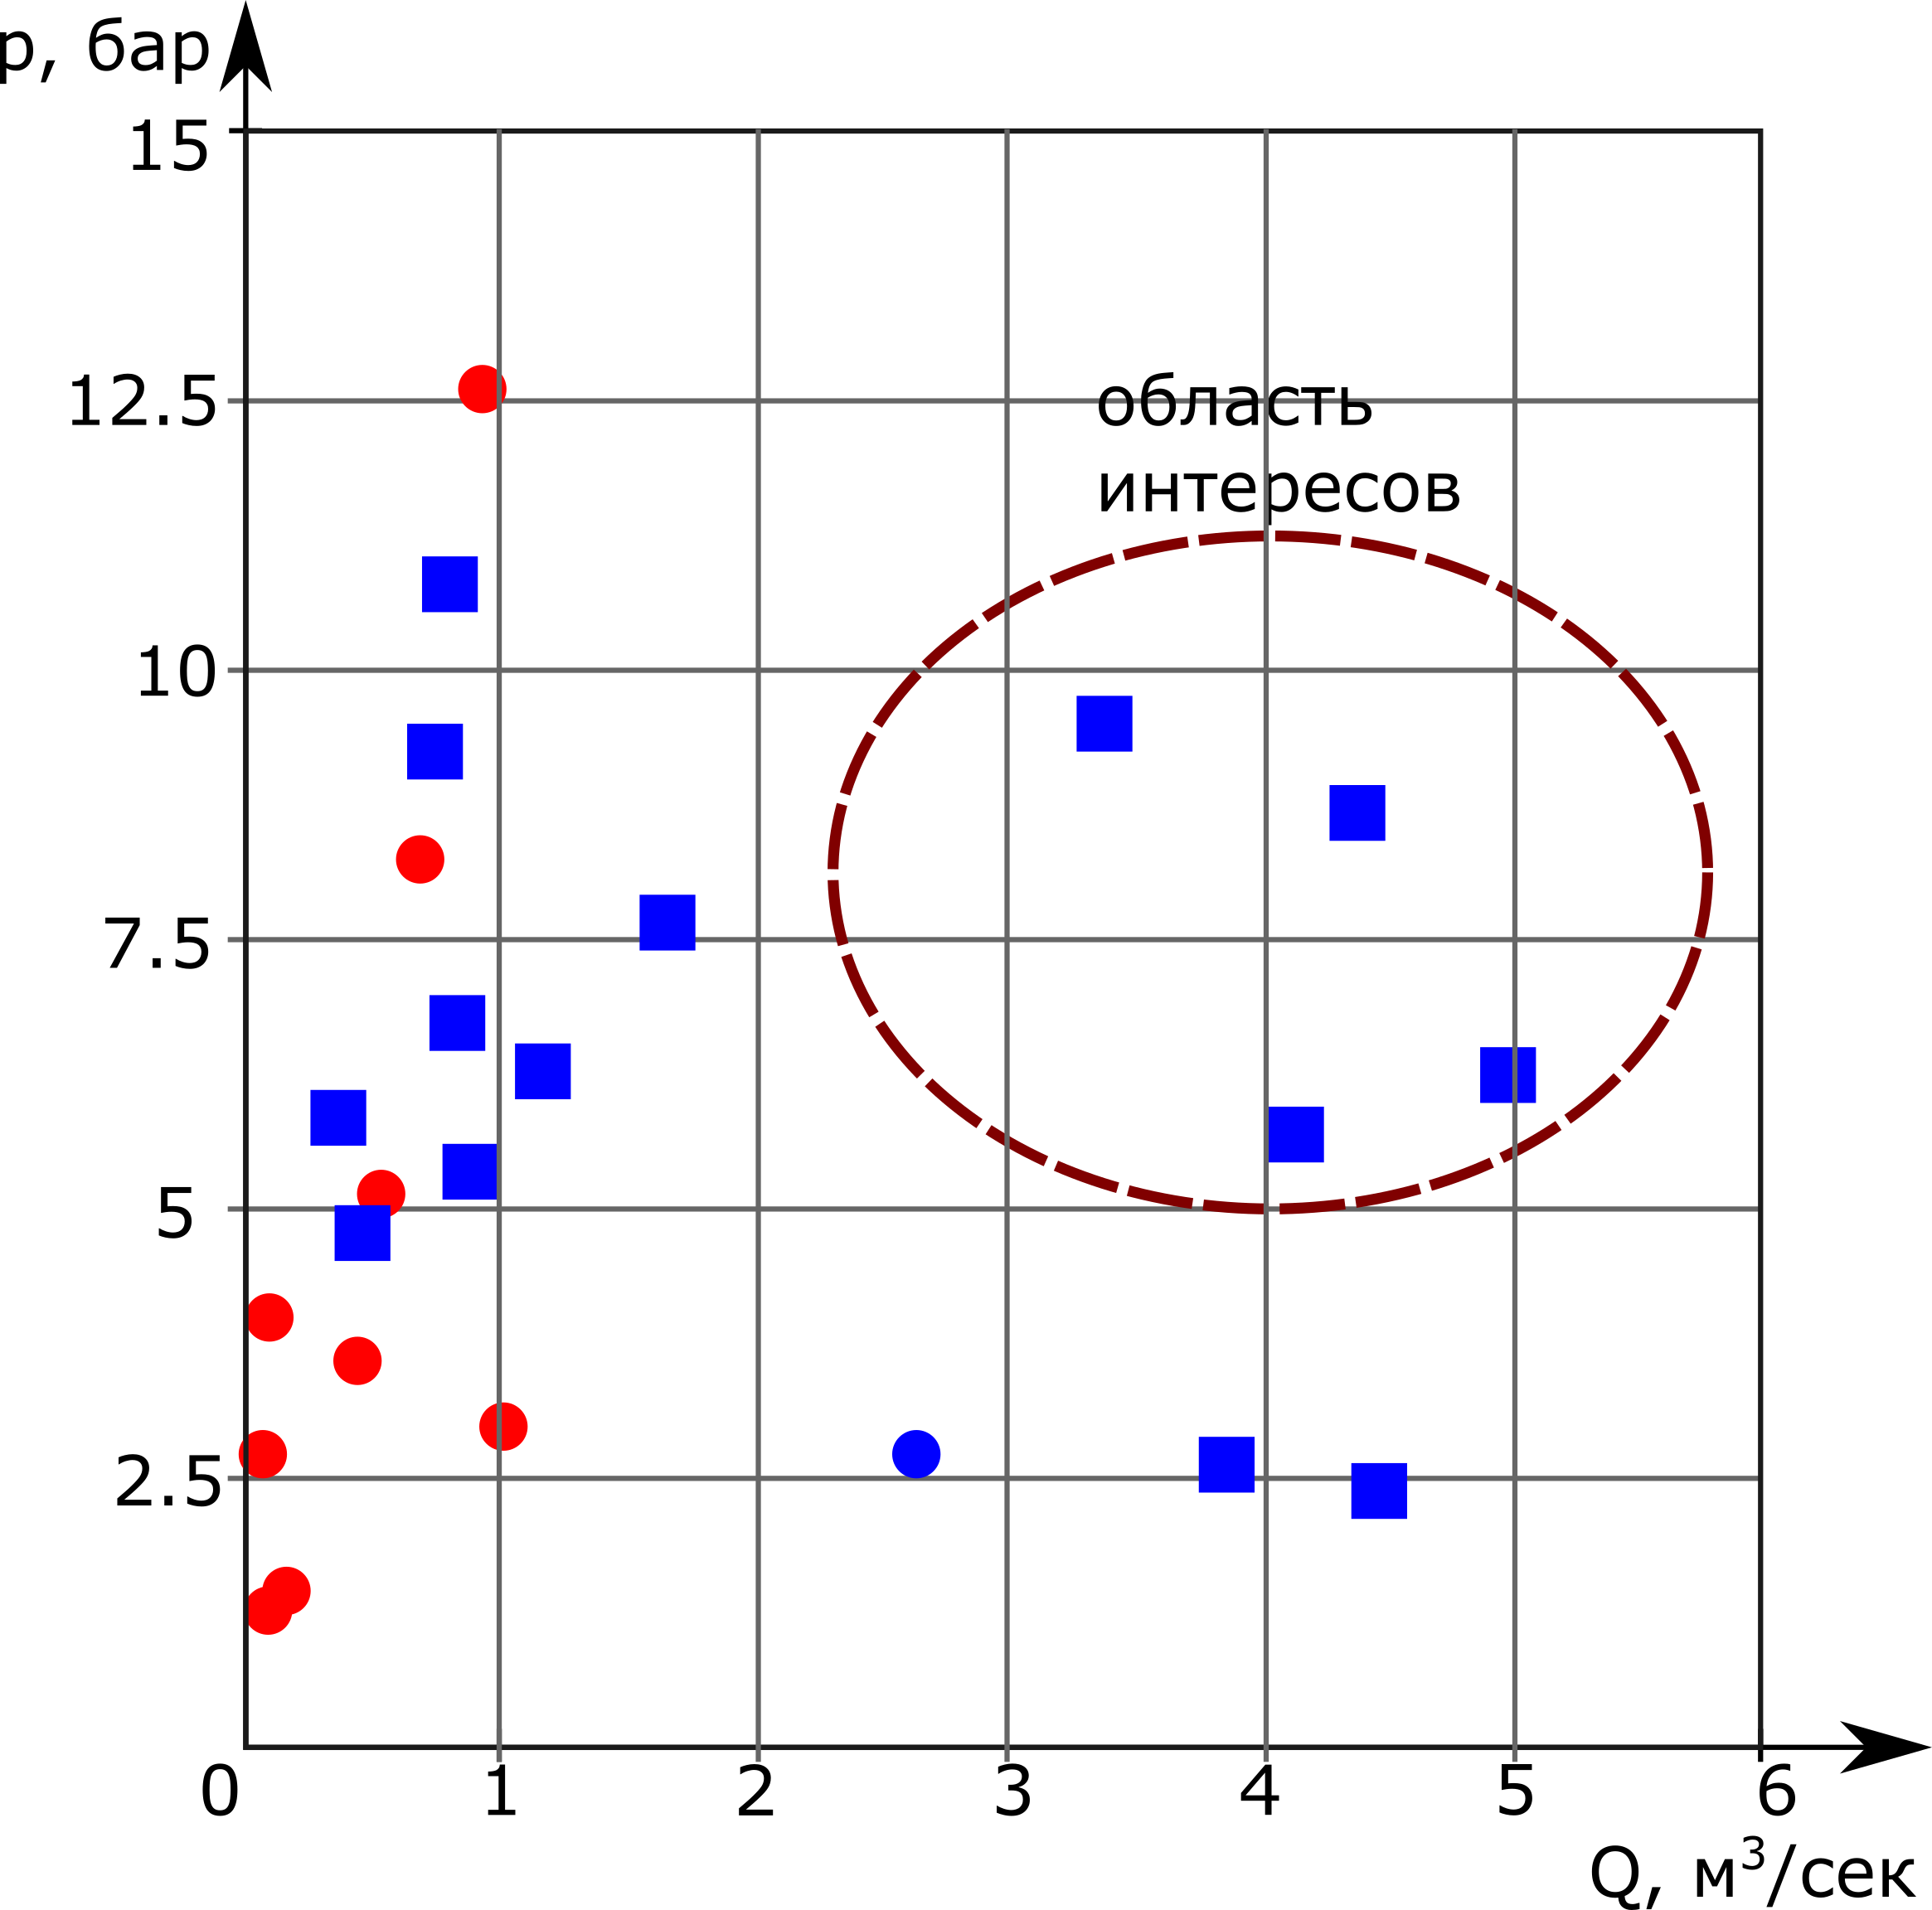
\includegraphics[width=0.45\textwidth]{Synopsis/images/part1/pQ_ru.png}
	\caption{Сравнение разработанных конструкций механических (синий цвет) и индукционных насосов (красный цвет).}
	\label{fig:intreting_pq}	
\end{wrapfigure}
Электромагнитные процессы применяются во множестве промышленных процессов металлургии, ядерной энергетики, термоядерного синтеза и т.д. Одна из основных современных проблем в этих областях -- это точность предсказания устойчивости потока жидкости под воздействием магнитного поля. Например, при проектировании индукционных насосов в диапазоне показанном, на Рис.~\ref{fig:intreting_pq}, возникают сильные турбулентные течения. Эти течения существенно влияют на показатели установки, снижают срок службы и приводят к аварийным режимам. С точки зрения гидродинамики такие режимы, их называют неустойчивыми, вызывают обратные течения, вихри потока жидкости, пульсации давления с двойной частотой магнитного поля и ряд других эффектов. Условие возникновения неустойчивых потоков можно выразить через производные разности давлений магнитного поля $\Delta \widetilde{p}_{эм}(\widetilde{Q}) = \frac{1-\widetilde{Q}}{1+Rm^2 (1-\widetilde{Q} )^2}$  и разности гидродинамического $\Delta \widetilde{p}_{ж} = \widetilde{Q}^n / N_s $ от расхода жидкости $\widetilde{Q}$, записанные в безразмерном виде

\begin{equation*}
    \frac{\partial (\Delta \widetilde{p}_{эм})} {\partial \widetilde{Q}} > \frac{\partial (\Delta \widetilde{p}_{ж})} {\partial \widetilde{Q}},
\end{equation*}
где число Стюарда определяется $N = \frac{\sigma B_{0}^2 U_{с} L}{2K_{n}}$ с помощью характерных значений пространства $L_0$, магнитной индукции $B_{0}$, скорости магнитного поля $U_{с}$, $\sigma$ - электропроводность среды и функция $K_{n}$, описывающая изменения давления в зависимости от скорости. После ряда математических преобразований можно записать условие неустойчивости с помощью неравенства, используя магнитное число Рейнольдса $R_{m}$ (\ref{eq:Rm}) и параметры гидродинамической системы, описывающиеся удельным расходом $\widetilde{Q}$ и функция поведения потока $K_n$, где $n$ зависит от поведения потока. 
\begin{equation}
    R_m > \frac{1}{1-\widetilde{Q}} \sqrt{\frac{n+(1-n) \widetilde{Q}}{(n+1)\widetilde{Q}-n}}.
    \label{eq:Rm}
\end{equation}
Из выражения $B = B_{0} / (j + R_{m}s)$ для бегущего магнитного поля со скольжением $s$ можно заключить, увеличение давления за счет повышения магнитной индукции приведет к  неустойчивым режимам потока жидкости. В таких режимах возникают сильные обратные течения, значительные колебания давления и ряд других эффектов опасных для экплуатации установки и делающих невозможным достигнуть требуемого диапазона характеристики изображенных на Рис.~\ref{fig:intreting_pq}. 

В этой части работы обсуждаются механизмы появления неустойчивости потоков, и что турбулентные течения описываются критическими значениями параметров, а их изменением во времени и пространстве, что делает возможным прийти к одному и тому же режиму работы различными способами, обойдя зоны в которых возникают турбулентные течения. Эти исследования требуют многокритериального анализа, который можно существенно упростить, используя $\pi$-теорему и теорию подобия. В этой работе исследования в большинстве случаев рассматриваются в безразмерном виде, с использованием числа подобия Рейнольдса $Re= U_{0} L_{0}/ \nu$, Гартмана $Ha = B_{0} L_{0} \sqrt{\sigma/ \rho \nu}$, Стюарта и магнитного Рейнольдса, а также их вариации для ряда задач и типа магнитного поля. 


\underline{\textbf{Вторая глава}} посвящена разработке процедуры решения уравнения момента (\ref{eq:moment}) и закона сохранения массы $ \nabla \cdot \mathbf{U} = 0$ несжимаемых жидкостей совместно с электромагнитными усилиями $\mathbf{F}$.
\begin{equation}
	\frac{\partial\mathbf{U}}{\partial t} +\left( \nabla \cdot \mathbf{U} \right) \mathbf{U} - \left( \nu + \nu_t \right) \Delta \mathbf{U} = -\nabla \frac{p}{\rho} + \frac{\mathbf{F}}{\rho},
	\label{eq:moment}
\end{equation}
В уравнении (\ref{eq:moment}) переменные обозначаются следующими символами  $\mathbf{U}$ скорость, $\nu$ -- кинематическая вязкость, $\nu_{t}$-- турбулентная кинематическая вязкость, $\rho$ -- плотность и $p$ -- давление. 
Для задач массо- и теплопереноса рассматриваемых данной работе уравнения момента (\ref{eq:moment}) и сохранения массы записываются для модели сжимаемой жидкости, а также добавляются уравнение энергии для расчета тепловых процессов и условия агрегатного состояния фракции. Эти все уравнения разрешаются в программе с открытой лицензией OpenFOAM. Электромагнитные усилия в \ref{eq:moment} вычисляются с помощью метода конечных элементов в программе Elmer. Во всех задачах магнитное поле представляется в гамоническом виде и описывается $A-\varphi$ формулировкой в комплексном виде с помощью векторного $\mathbf{\underline{A}}$ и скалярного $\underline{\varphi}$ магнитного потенциала, как
\begin{equation}
	\Delta \mathbf{\underline{A}}-j\omega \mu \sigma \mathbf{\underline{A}}-\mu \sigma \nabla \underline{\varphi}+\mu \sigma (\mathbf{U}\times \nabla \times \mathbf{\underline{A}})=-\mu \mathbf{\underline{J}},	
	\label{eq:Aphi}
\end{equation}
где $\mu$ - абсолютная магнитная проницаемость среды, $\sigma$ -- электропроводность, $\omega$ -- угловая частота.
 
\begin{wrapfigure}{l}{0.4\textwidth}
	\centering
	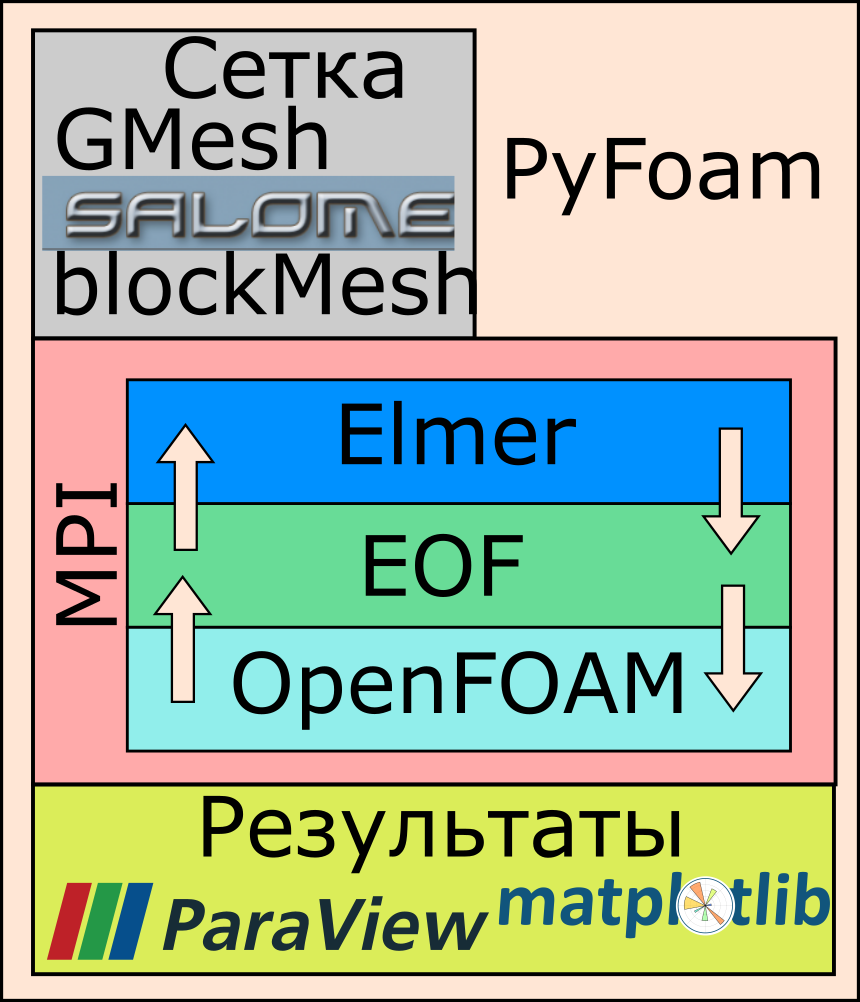
\includegraphics[width=0.3\textwidth]{Synopsis/images/part2/GeneralChartFlow_ru.png}
	\caption{Структурная схема взаимодействия программ для расчета задач.}
	\label{fig:solver}	
\end{wrapfigure}
Исследование механизмов возникновения неустойчивых режимов потока жидкости требует большого количества перебора параметров и изменение настроек модели. Также работа с программами с открытой лицензией требует большого количества рутинных манипуляций с текстовыми файлами для настройки модели. С целью экономии времени для настройки модели, осуществления параметрических исследований и сокращения рутинных операций была написана библиотека PyRunOF
на языке  Python и доступная в открытом доступе на репозитории gitHub \footnote{https://github.com/TreeDa93/PyRunOF}. Основные ее возможности -- это создавать расчетную область и дискретизировать ее с помощью пакетов Salome, Gmesh или встроенной утилиты blockMesh в OpenFOAM; задавать начальные и граничные условия, переносить их из результатов других моделей; определять параметры исследования, запускать на расчет мультифизиеские модели с помощью библиотеку EOF-library, а также производить обработку результатов в программе ParaView или python библиотеке matplotlib. Блок--схема алгоритма работы этой библиотеки указана на Рис.~\ref{fig:solver}. 

Верефикация рассматриваемых в работе моделей и алгоритмов решений уравнений магнитной гидродинамики была проведена с помощью сравнения с результатами получеными аналитическим способом и встроенной процедурой решения <<mhdFoam>> в программе OpenFOAM для вариации задачи Гартамана в двухмерной постановке Рис.~\ref{fig:comparision}, а. 
Важность учета всех размерностей пространства и корректного выбора граничных условий в моделях показана с помощью сравнения распределения скорости двухмерных и трехмерных моделей 
для случаев (см. Рис.~\ref{fig:comparision}), б: (а) -- все стенки изолированные; (б) -- стенки, перпендикулярные направлению магнитного поля, обладают бесконечной проводимостью, а стенки, параллельные магнитному полю, изолированы; (в) -- все стенки обладают бесконечной проводимость. Производительность рассматриваемого кода сравнена с расчетами получеными в программах полученными в коммерческих пакетах Comsol и ANSYS (Таблицу~\ref{tab:comparision}). Помимо оценки производительности был проведен анализ точности получаемых результатов с помощью сравнения с результатами из коммерческих программам для тестовых задач и данных из эксперемента для трехфазного перемешивателя, в котором скорость измеряется доплеровским датчиком.


\begin{figure}[t]
	\centerfloat{
	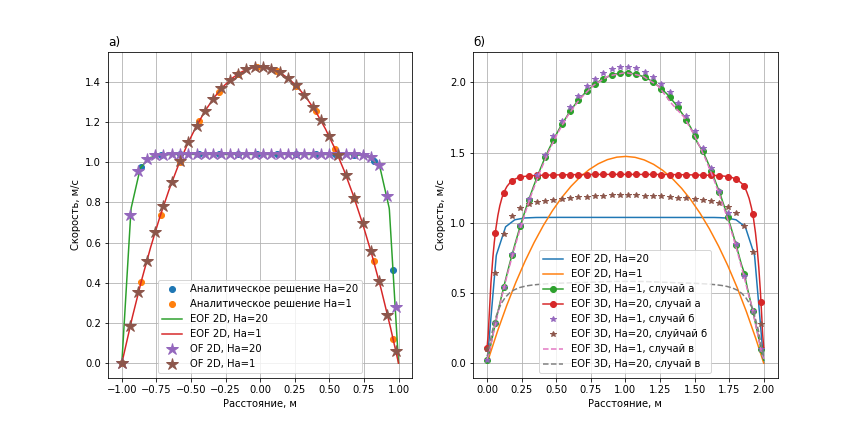
\includegraphics[width=1\linewidth]{Synopsis/images/part2/2D_comparisions.png}
	}
	\caption{Сравнение распределения скорости между стенками перпендикулярными магнитному полю а) сравнение разных подходов к решению двухмерной постановки задачи при числах Гартмана 1 и 20; б) результаты полученные с помощью решателя EOF для двухмерной и трехмерной постановки задачи при числах Гартмана 1 и 20.}
	\label{fig:comparision}
	
\end{figure}

\begin{table}[h!]
	\centering
	\captionsetup{justification=centering}
	\caption{Сравнение времени расчета задачи потока проводящей жидкости в прямоугольном канале под воздействием магнитного поля в различных численных пакетах}
	\begin{tabular}{llccllcc}
		\toprule	
			Программный пакет & 2 ядра        & 4 ядра       & 8  ядер    & 12   ядер  \\
			\midrule
			OpenFOAM                       & 250 сек  & 132 сек  & 89 сек  & 93 сек  \\ \hline
			Библиотека EOF                 & 1992 сек & 1080 сек & 757 сек & 639 сек \\ \hline
			Comsol                         & 250  мни & -        & 48 мин  & -       \\ \hline
			ANSYS                          & 40 мин   & -        & 30 мин  & -       \\ \hline
	\end{tabular}
\label{tab:comparision}
\end{table}



\underline{\textbf{Третья глава}} посвящена исследованию влияния магнитных эффектов на поведения потока в различных режимах работы в прямоугольном канале \fixme{100мм x 100мм x 500 мм} (см. Рис.~\ref{fig:model}). Размер канала выбран для удобства расчета безразмерных чисел, а результаты могут быть масштабированы с высокой точностью на другие размеры каналов.  На расстоянии 100 мм от каждой стенки действует магнитное поле перпендикулярное направлению движения потока жидкости. 
\begin{wrapfigure}{l}{0.6\textwidth}
	\centering
	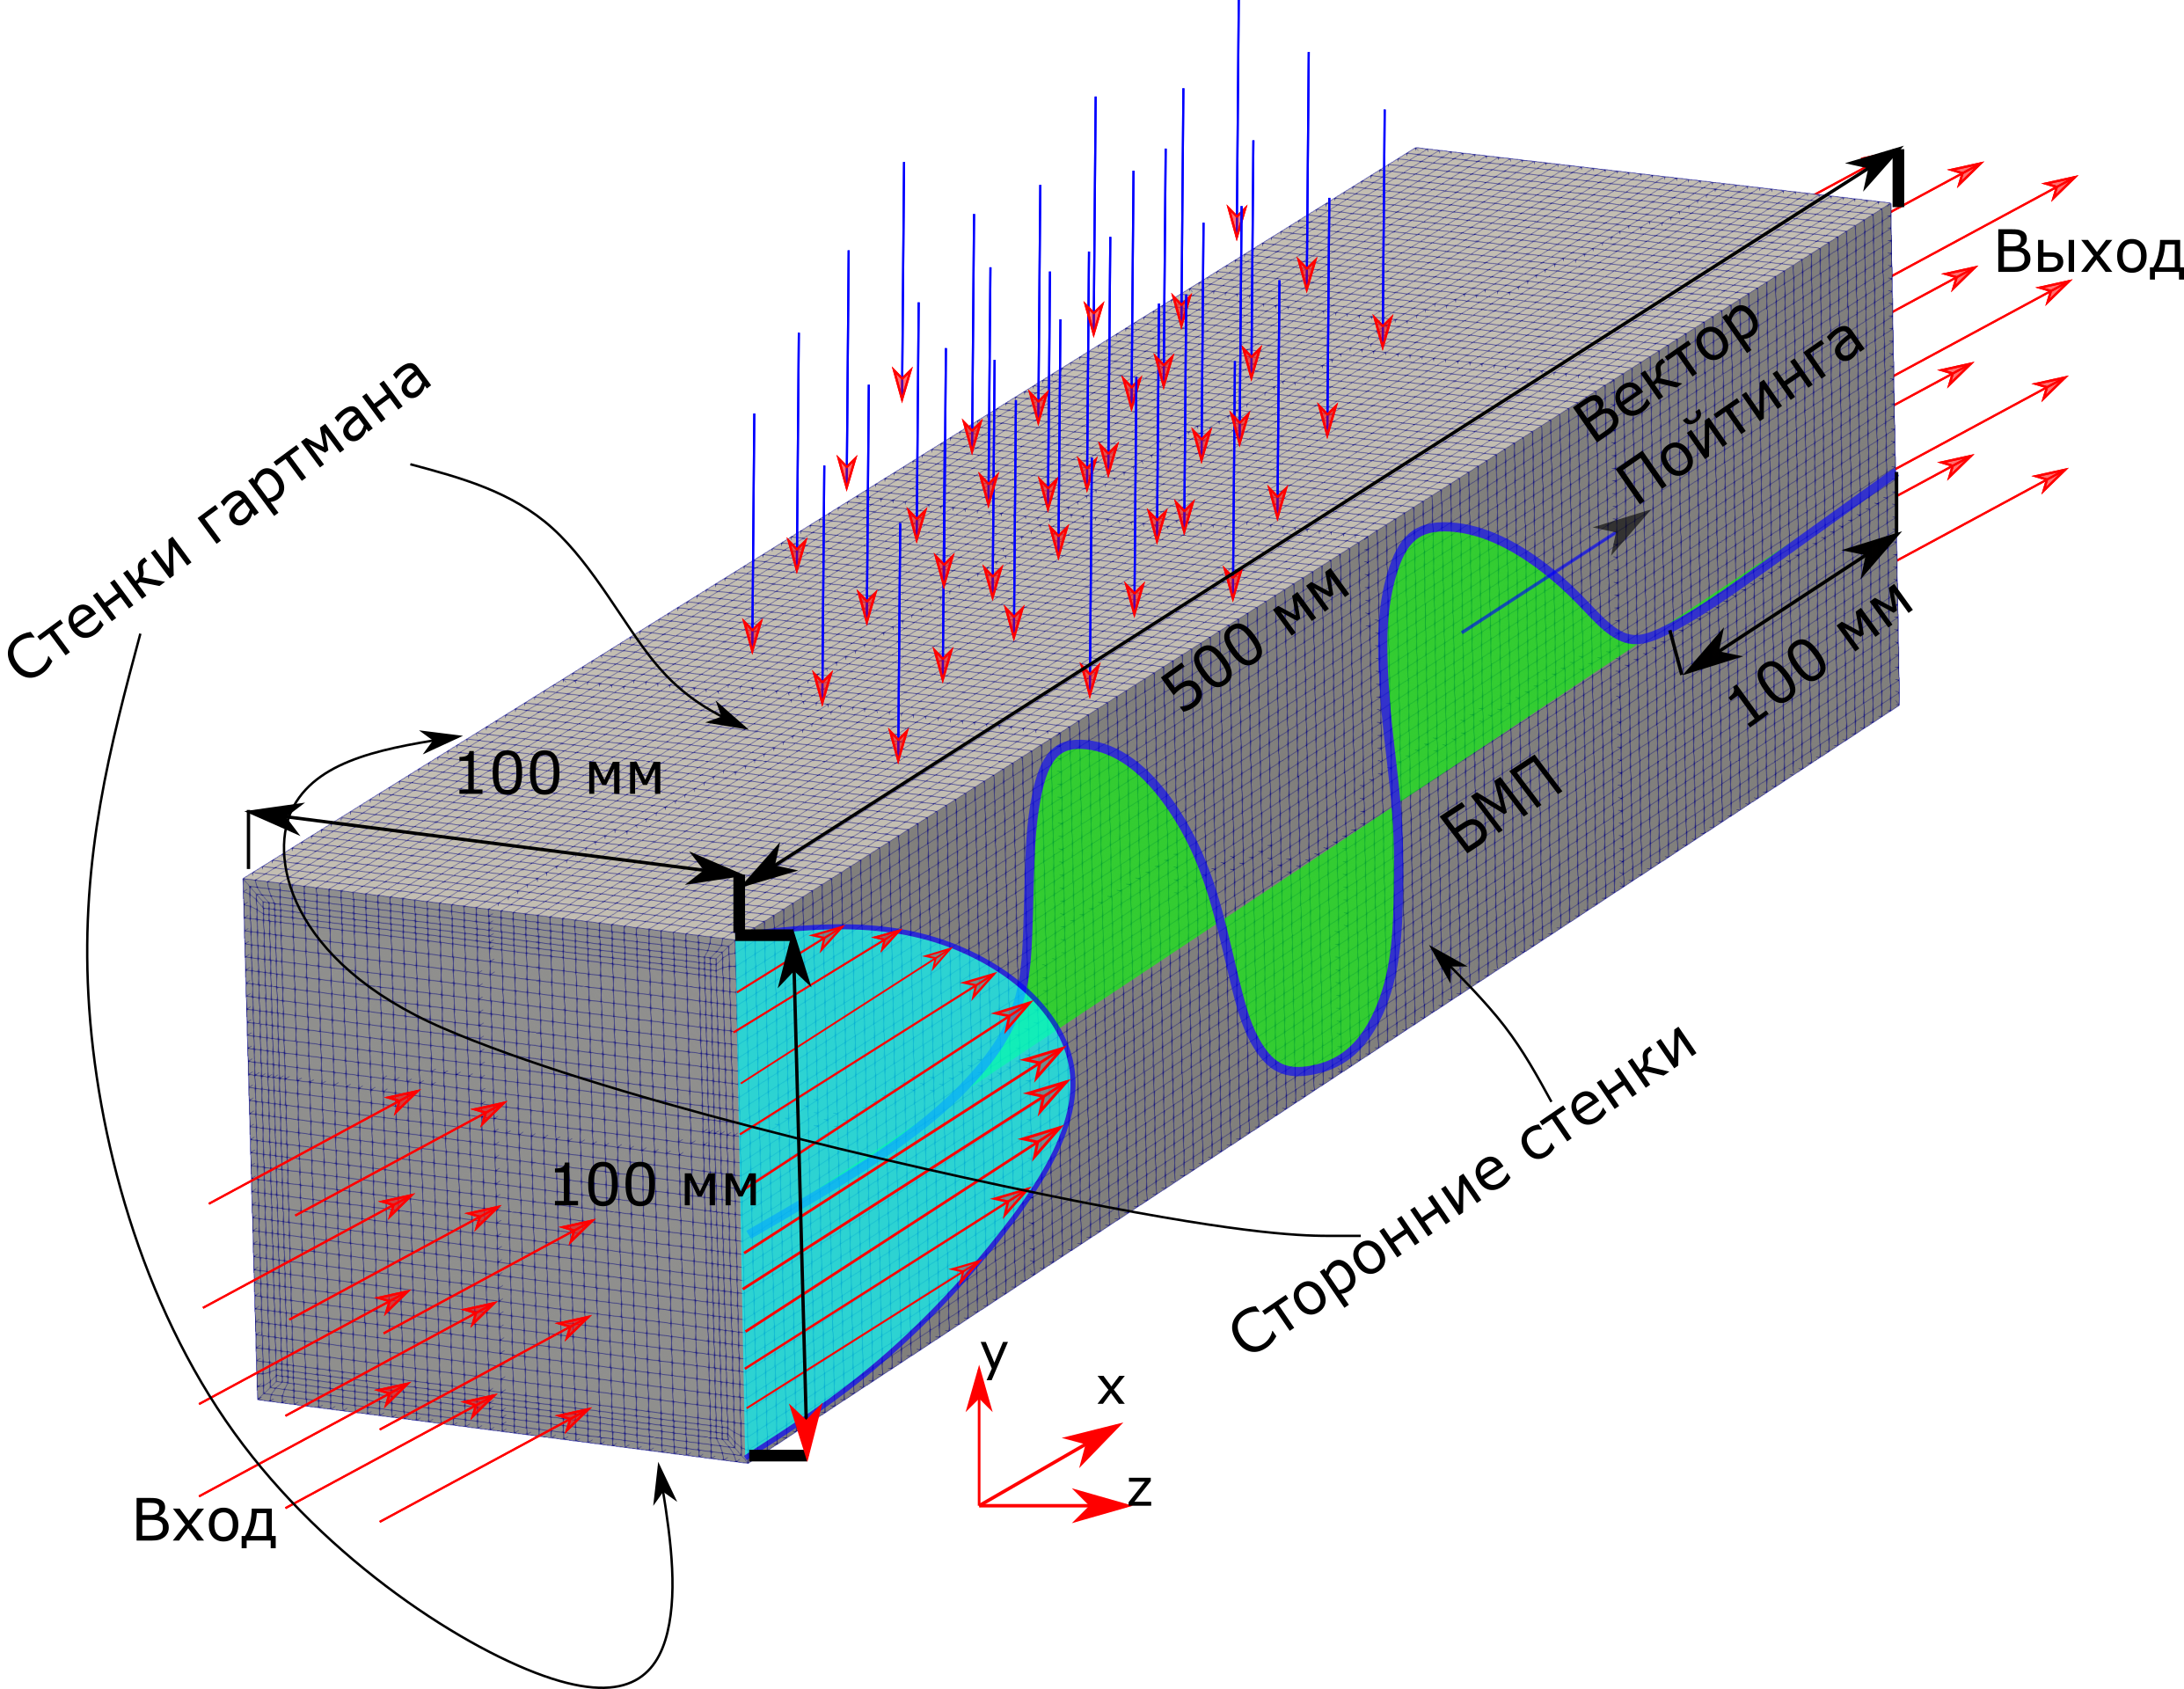
\includegraphics[width=0.55\textwidth]{Synopsis/images/part3/Description_ru.png}
	\caption{Описание модели.}
	\label{fig:model}	
\end{wrapfigure}
Магнитное поле описывается уравнением $\underline{\mathbf{B}} = \mathbf{B} e^{j(\omega - \varphi - \alpha x)}$. Для имметации конечности магнитной системы магнитное поле отсутсвует на растоянии 100 мм от входа и выхода канала. В модели стенки рассматриваются идеально изолированными $grad \varphi = 0$ для электрического тока и без проскальзывания $\mathbf{U} = 0$ для потока жидкости. На входе канала задается граничное условие Пуазейлевское распределение скорости из ранее рассчитанной модели без магнитного поля. Начальные значения для остальных переменных заданы из предварительного расчета без магнитного поля. На выходе задается граничное условие нулевого давления.
Для сравнения влияния продольного и поперечно краевых эффектов на поведение потока, были разработаны четыре модели:
\begin{enumerate}
	\item Случай 1 -- идеализированное бегущее магнитное поле. Влияние индуцированных токов на изменение общей магнитной индукции не учитывается (эффект входа-выхода в особенности не учитывается). В расчетах участвуют только компоненты плотности токов, создающие тяговые усилия (продольный краевой эффект не учитывается);
	\item Случай 2 --  Влияние индуцированных токов на изменение общей магнитной индукции учитывается (эффект входа-выхода в особенности учитывается). В расчетах участвуют только компоненты плотности токов, создающие тяговые усилия (продольный краевой эффект не учитывается);
	\item Случай 3 -- Влияние индуцированных токов на изменение общей магнитной индукции учитывается (эффект входа-выхода в особенности не учитывается). В расчетах участвуют все три компоненты плотности токов, создающие усилия по трем направлениям (продольный краевой эффект учитывается);
	\item Случай 4 -- неидеализированное бегущее магнитное поле, учитывается поперечный и продольный краевой эффект.  
\end{enumerate}
Продольный краевой эффект был исключен из модели искусственным занижением электропроводности в расчетах для получения распределения плотности тока, но с пренебрежимо малыми значениями для влияния на общее магнитное поле. Затем при расчете поля скоростей в уравнеии моемента (\ref{eq:moment}) член усилий увеличивается в количетсво раз  на сколько была снижена электропроводность.

\begin{figure}[b]
	\centerfloat{
		\begin{subfigure}[b]{0.5\textwidth}
			\centering
			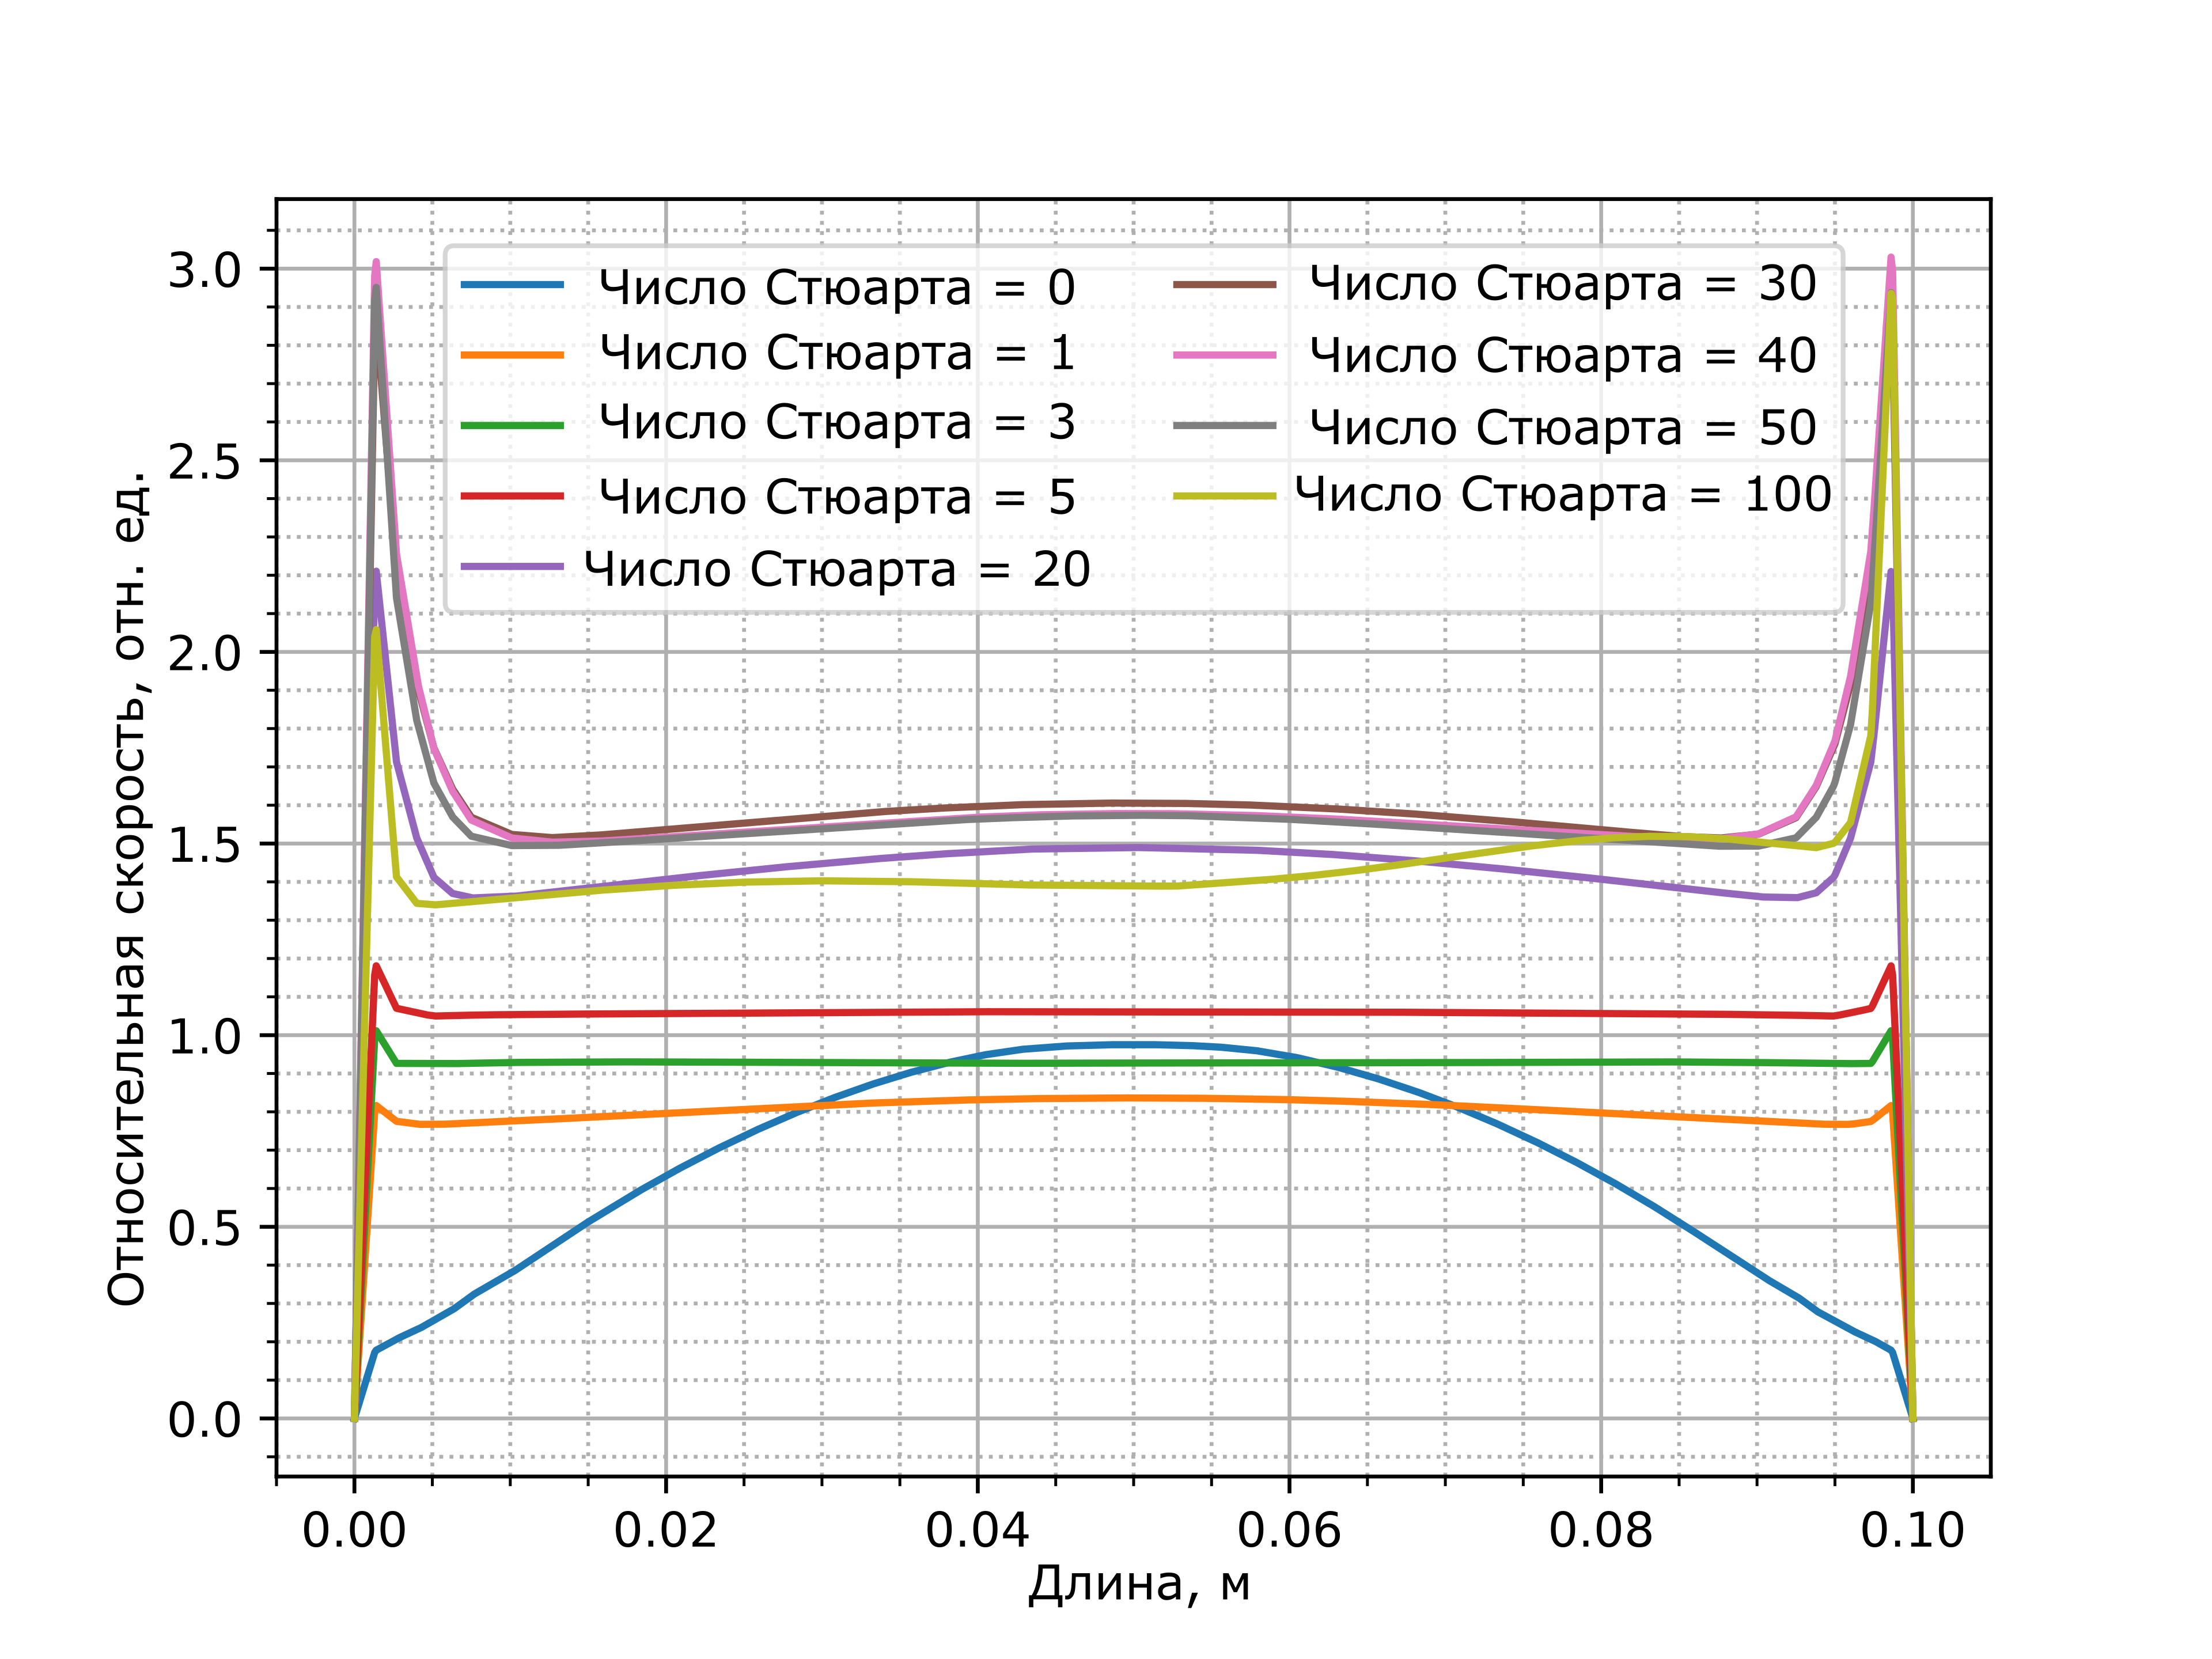
\includegraphics[width=\textwidth]{Synopsis/images/part3/ideal_velocity_z_ru.png}
		\end{subfigure}
		\hfill
		\begin{subfigure}[b]{0.5\textwidth}
			\centering
			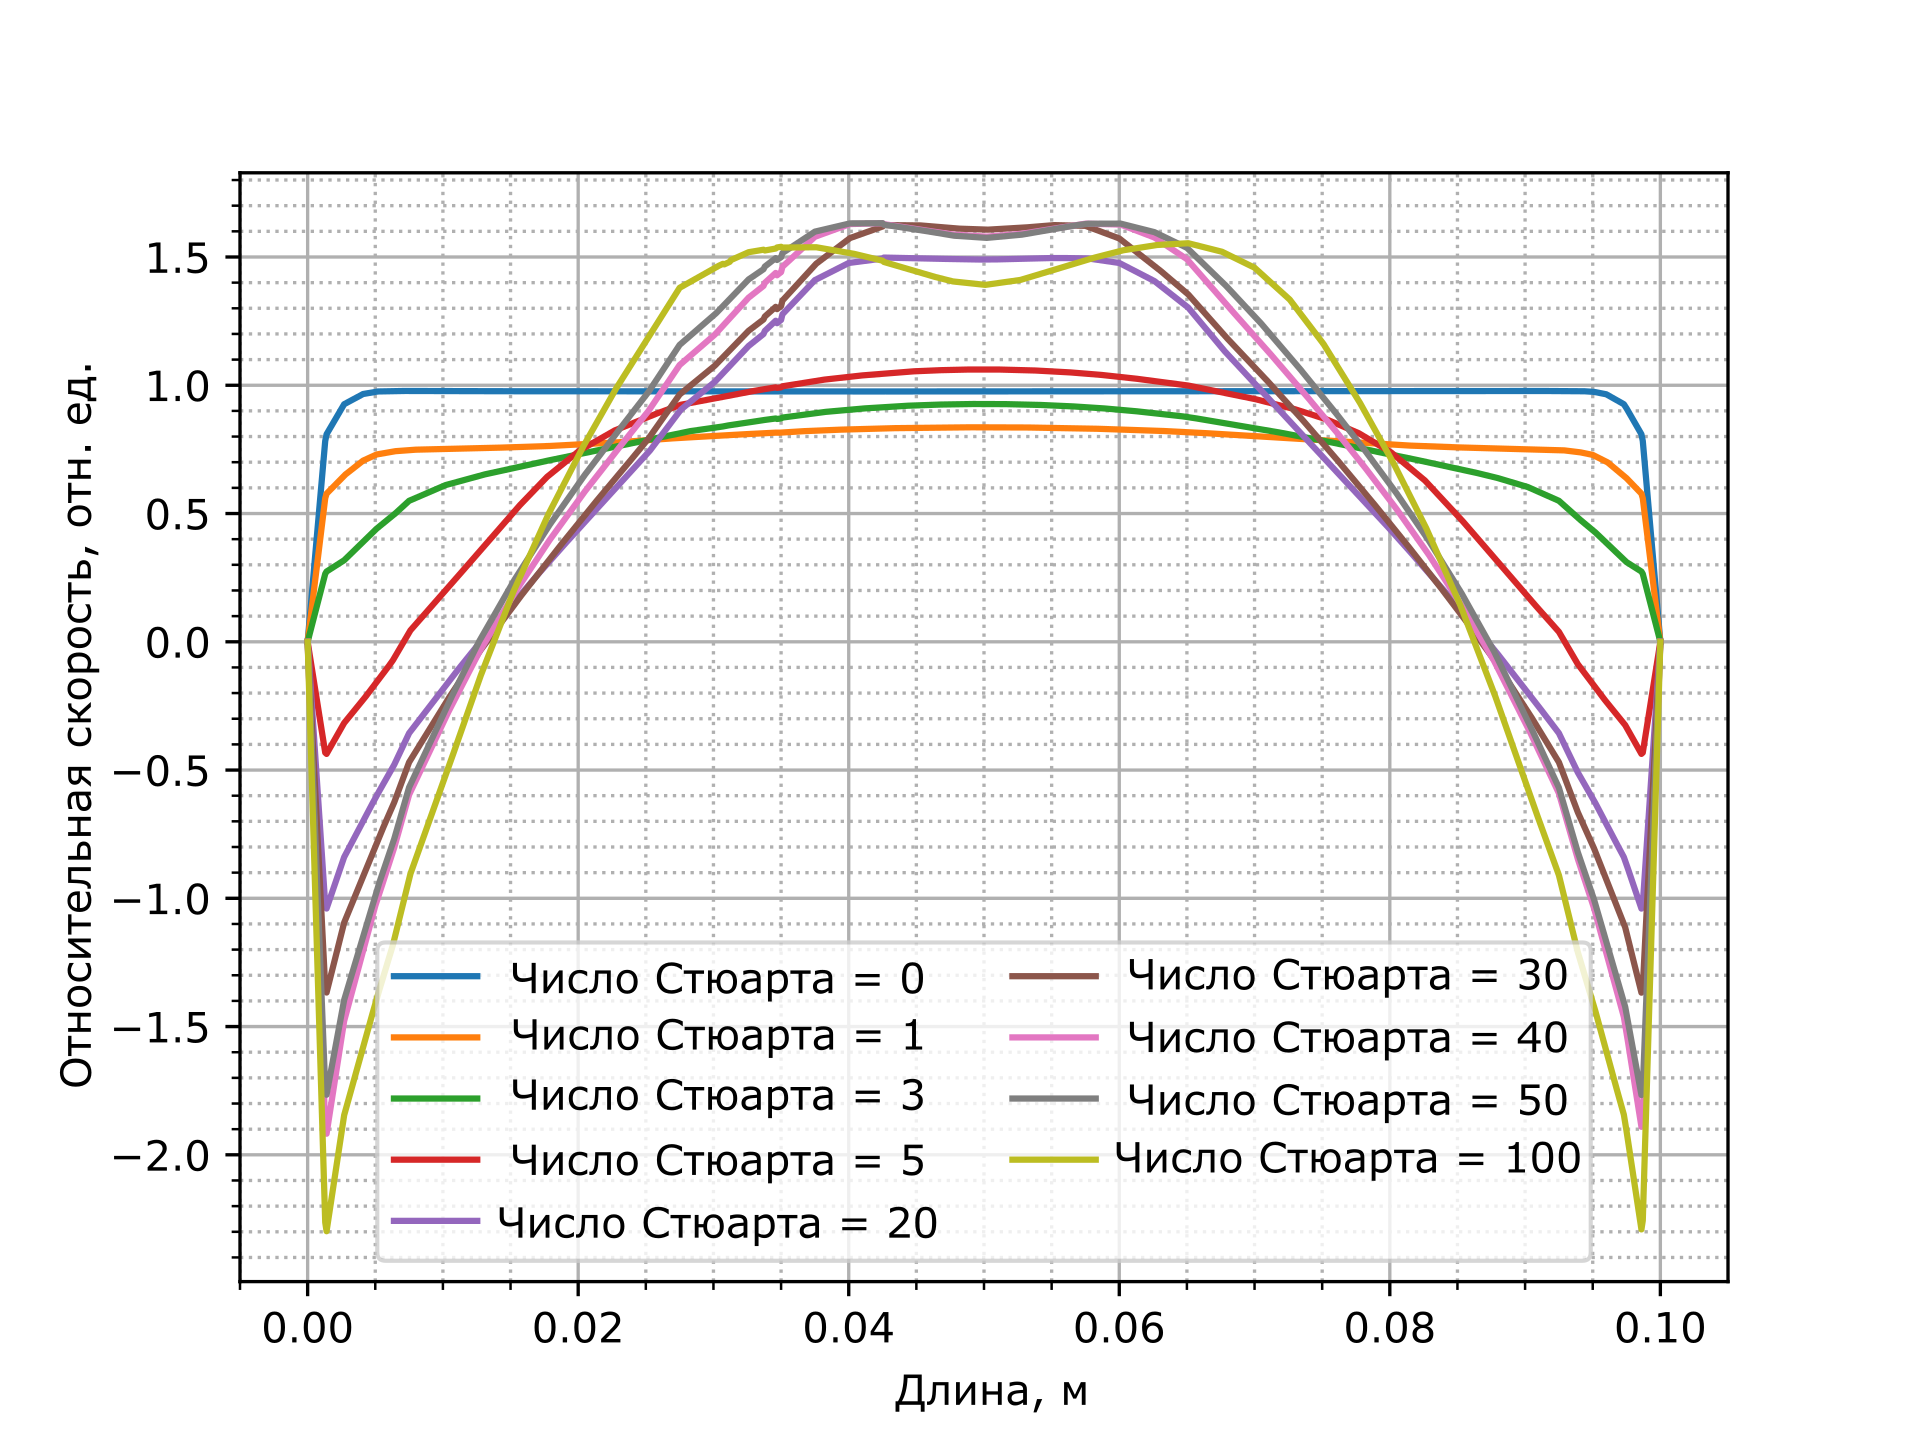
\includegraphics[width=\textwidth]{Synopsis/images/part3/ideal_velocity_Y_ru.png}
		\end{subfigure}
	}
	\caption{Распределение скорости между стенками: а) перпендикулярными магнитному полю и б) параллельными магнитному полю в центре канала.}
	\label{fig:velocity:ideal}
\end{figure}

На Рис.~\ref{fig:velocity:ideal} показаны графики удельной скорости вдоль линий в центре канала между стенками перпендикулярными (Рис.~\ref{fig:velocity:ideal}, а) и параллельными (Рис.~\ref{fig:velocity:ideal}, б) магнитным линиям для идеализированного бегущего магнитного поля (случай 1). Результаты показаны для постоянного числа Рейнольдса 54500,  числа Гартмана и Стюарда варьируется от 0 до 7377 и  от 0 до 100, соответсвенно. Можно заметить ускорение потока (небольшие пиковые значения скорости) у стенок перпендикулярных магнитному полю (гартмоновские) при малых значениях Стюарда от 0 до 5, в то время как на этих же числах Стюарта у стенок параллельных магнитному полю это ускорение отсутствует. Потоки с противоположной по значению скоростью основному потоку образуются у стенок параллельных магнитному полю, а у гартмоновских стенок значительное ускорение потока при числах Стюарда больше четырех. Обратные потоки существенно снижают эффективное сечение канала, что приводит к повышениею гидродинамической нагрузки. Можно отметить, что значения удельной скорости обратных потоков меньше, чем ускорения, но дистанция их распространения значительно больше., что приводит к сужению эффективного сечения в плоскости перендикулярной магнитному полю. 

\begin{figure}[b]
	\centering{
		\begin{subfigure}[b]{0.3\textwidth}
			\centering
			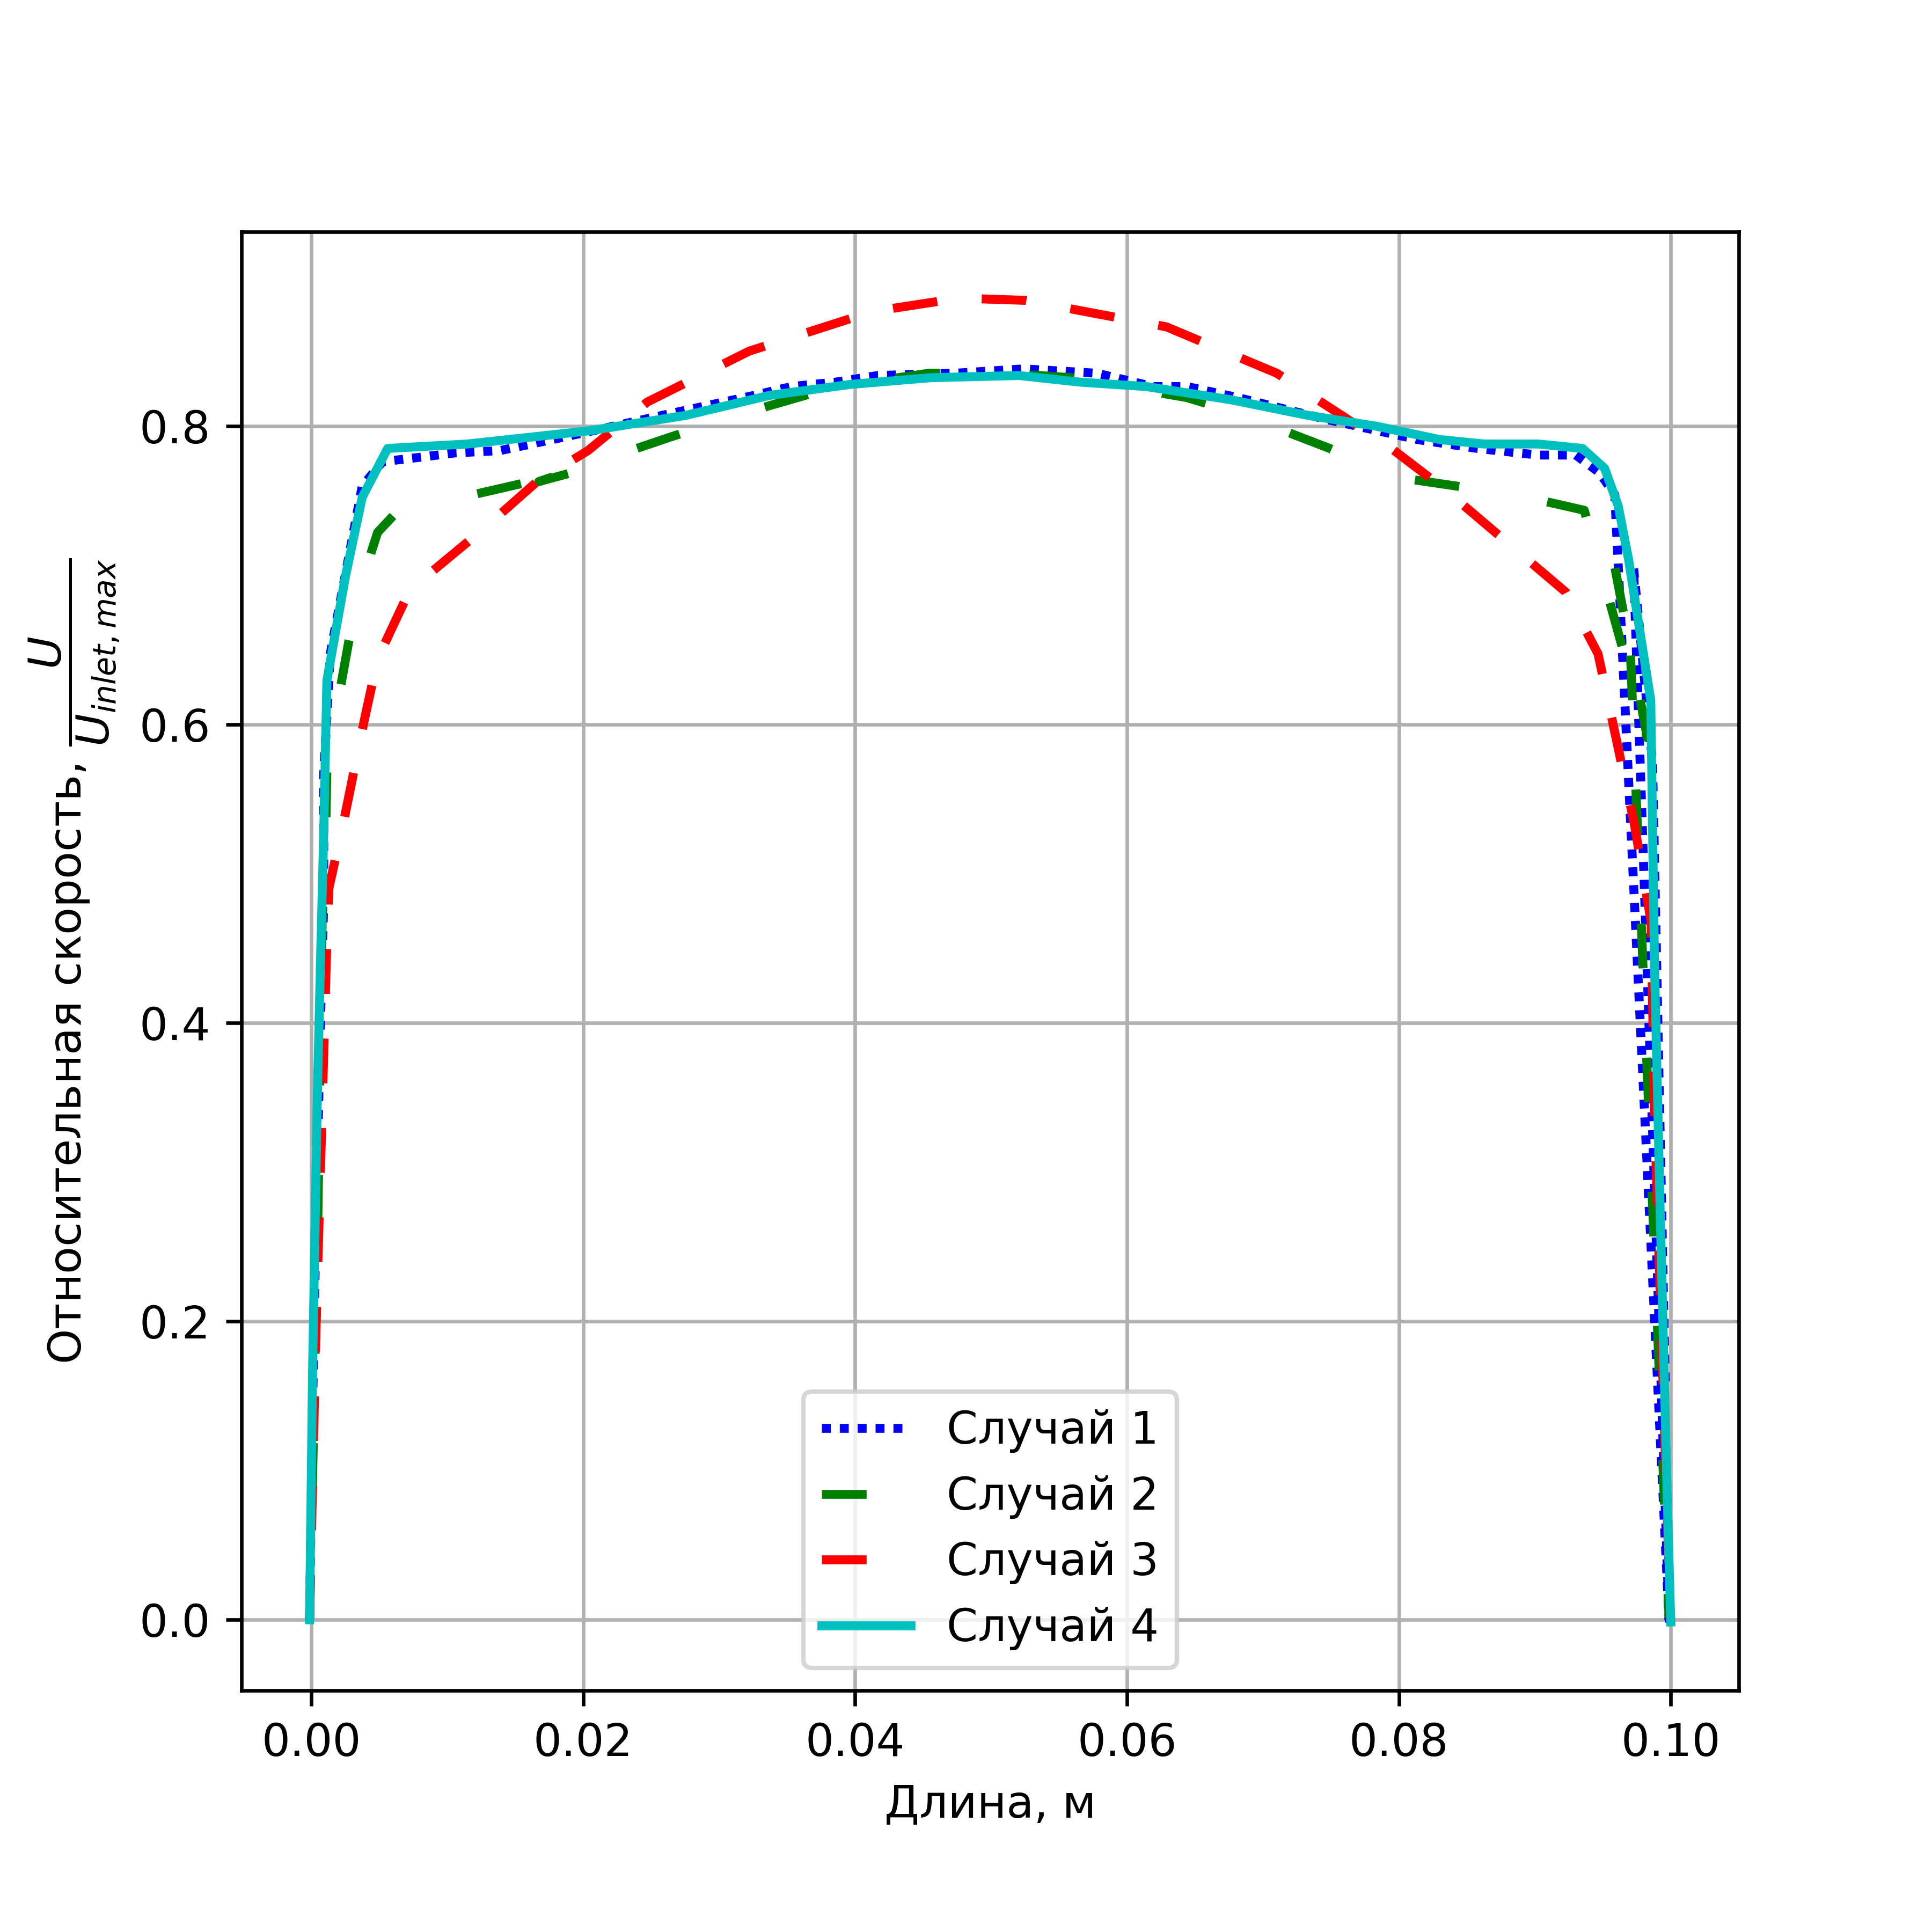
\includegraphics[width=\textwidth]{Synopsis/images/part3/y_velocity_st_1.png}
		\end{subfigure}
		\hfill
		\begin{subfigure}[b]{0.3\textwidth}
			\centering
			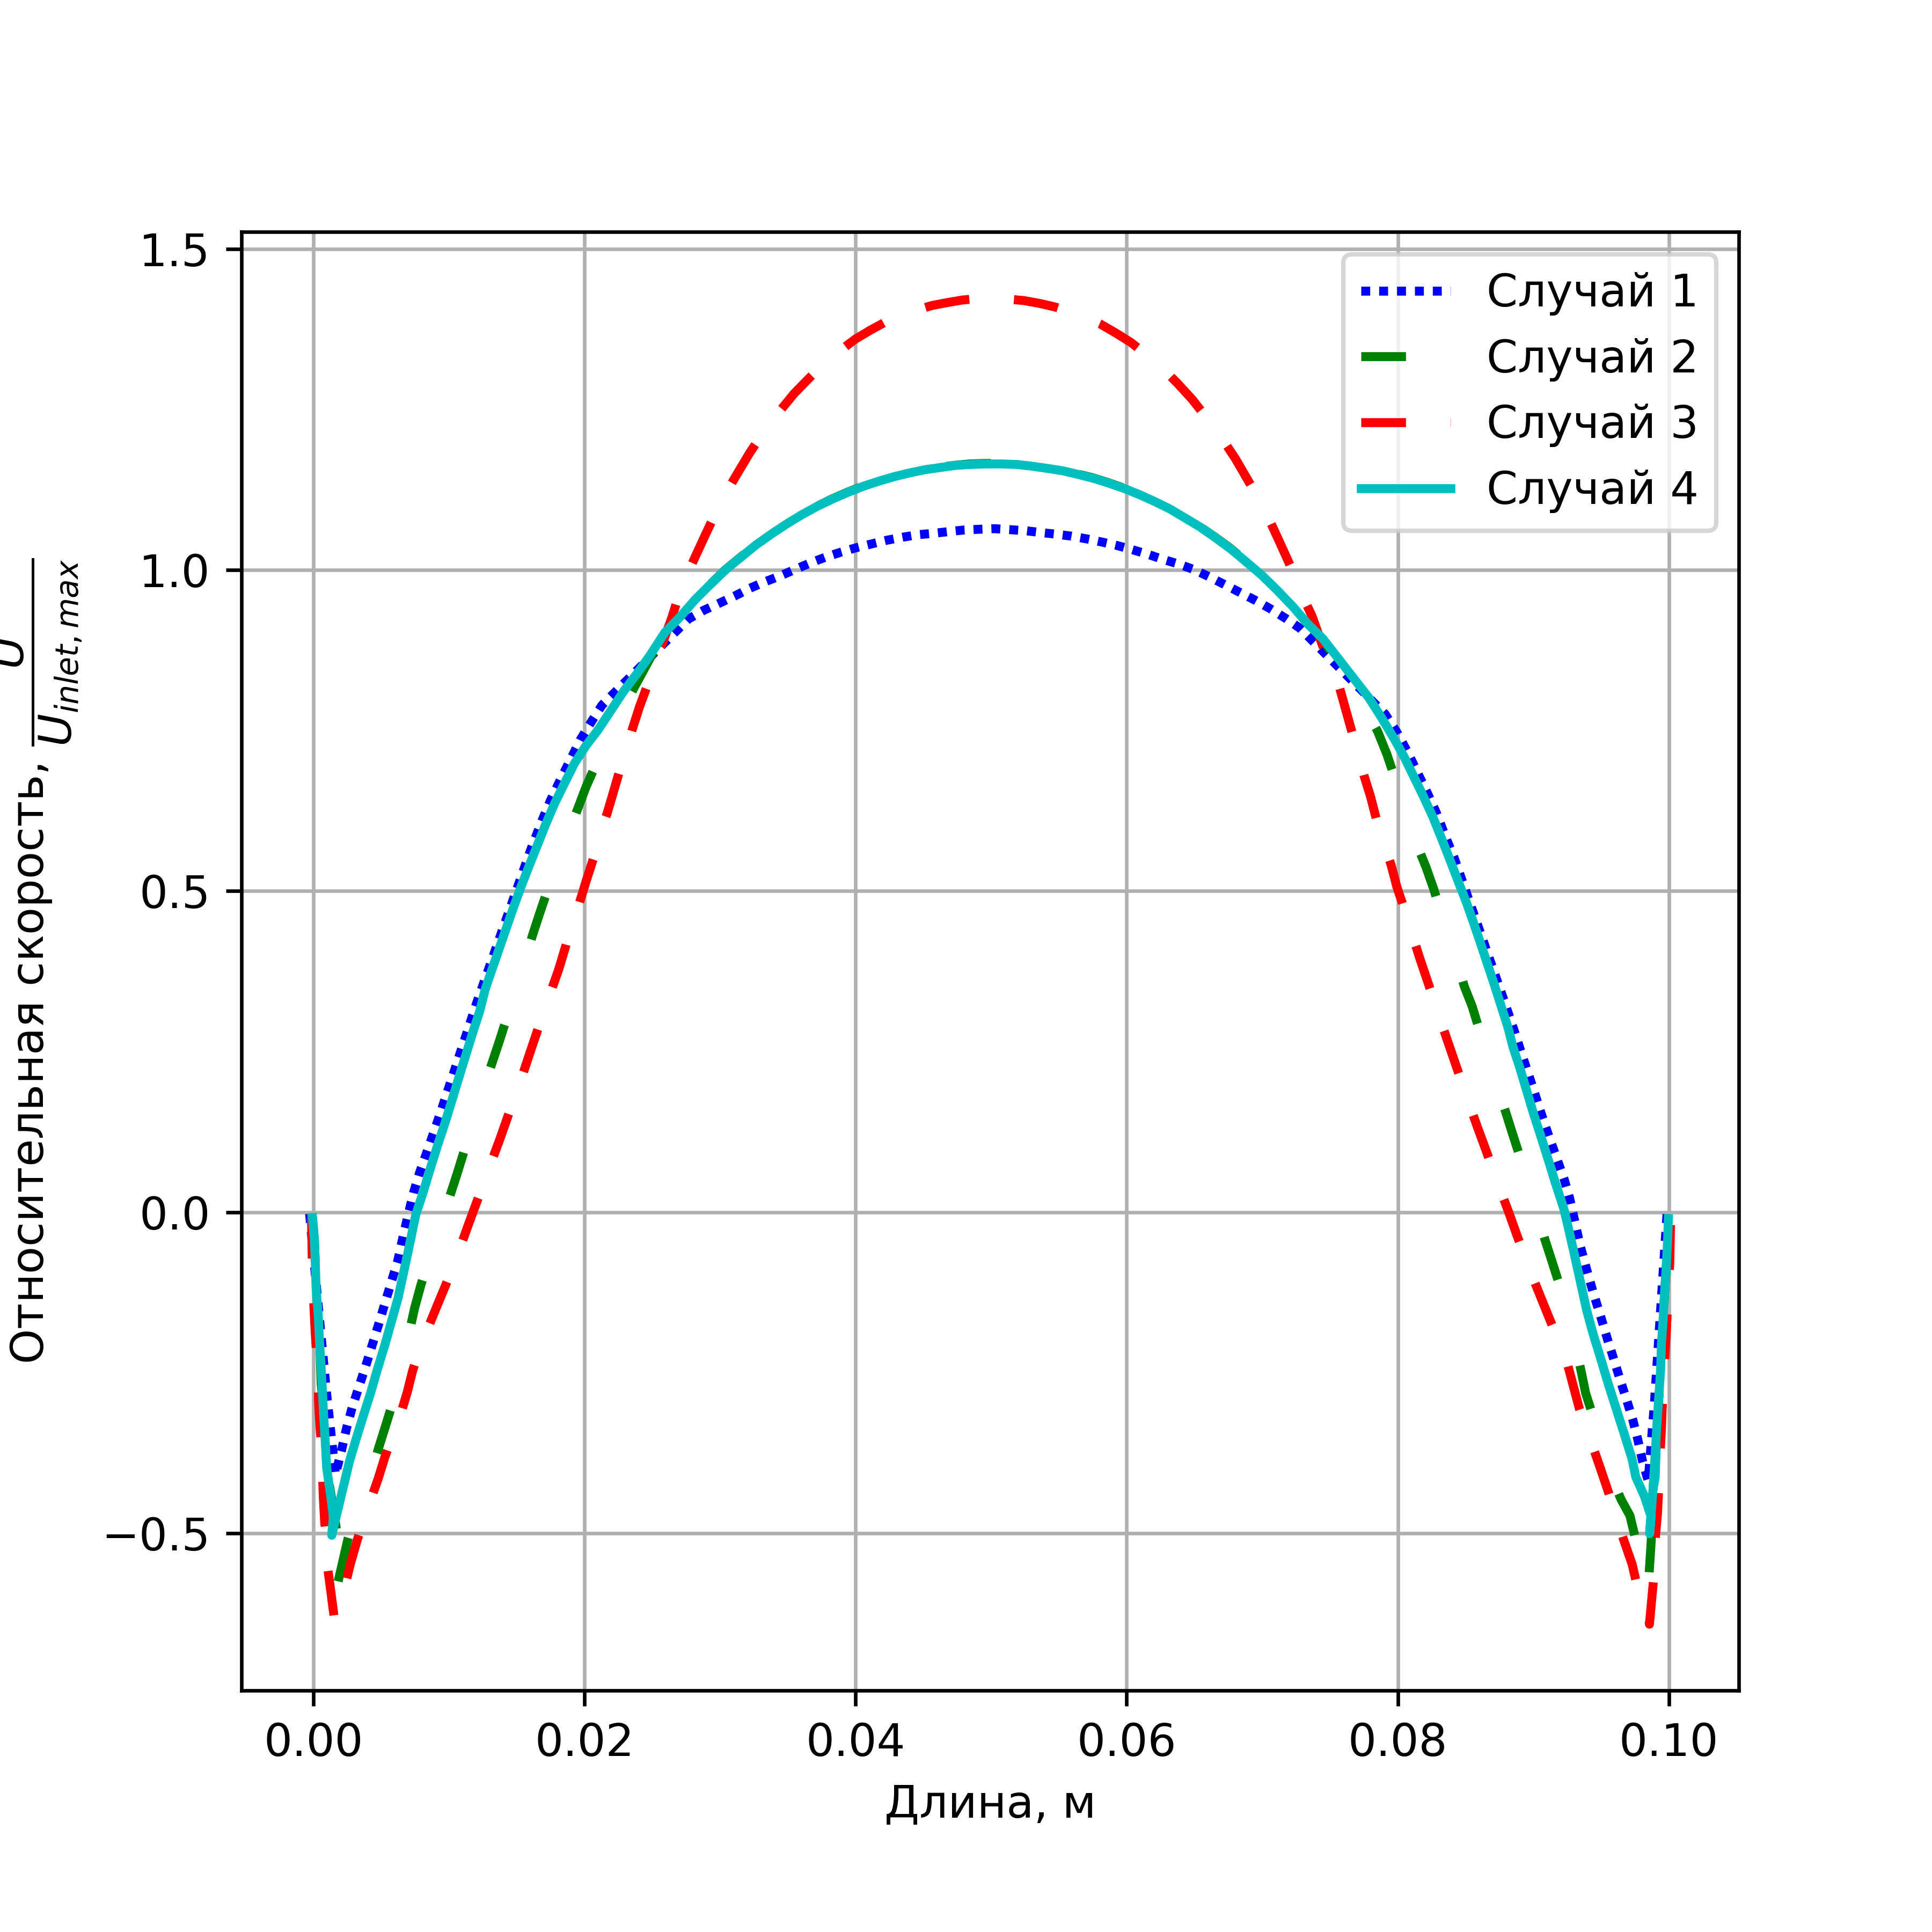
\includegraphics[width=\textwidth]{Synopsis/images/part3/y_velocity_st_5.png}
		\end{subfigure}
		\hfill
		\begin{subfigure}[b]{0.3\textwidth}
			\centering
			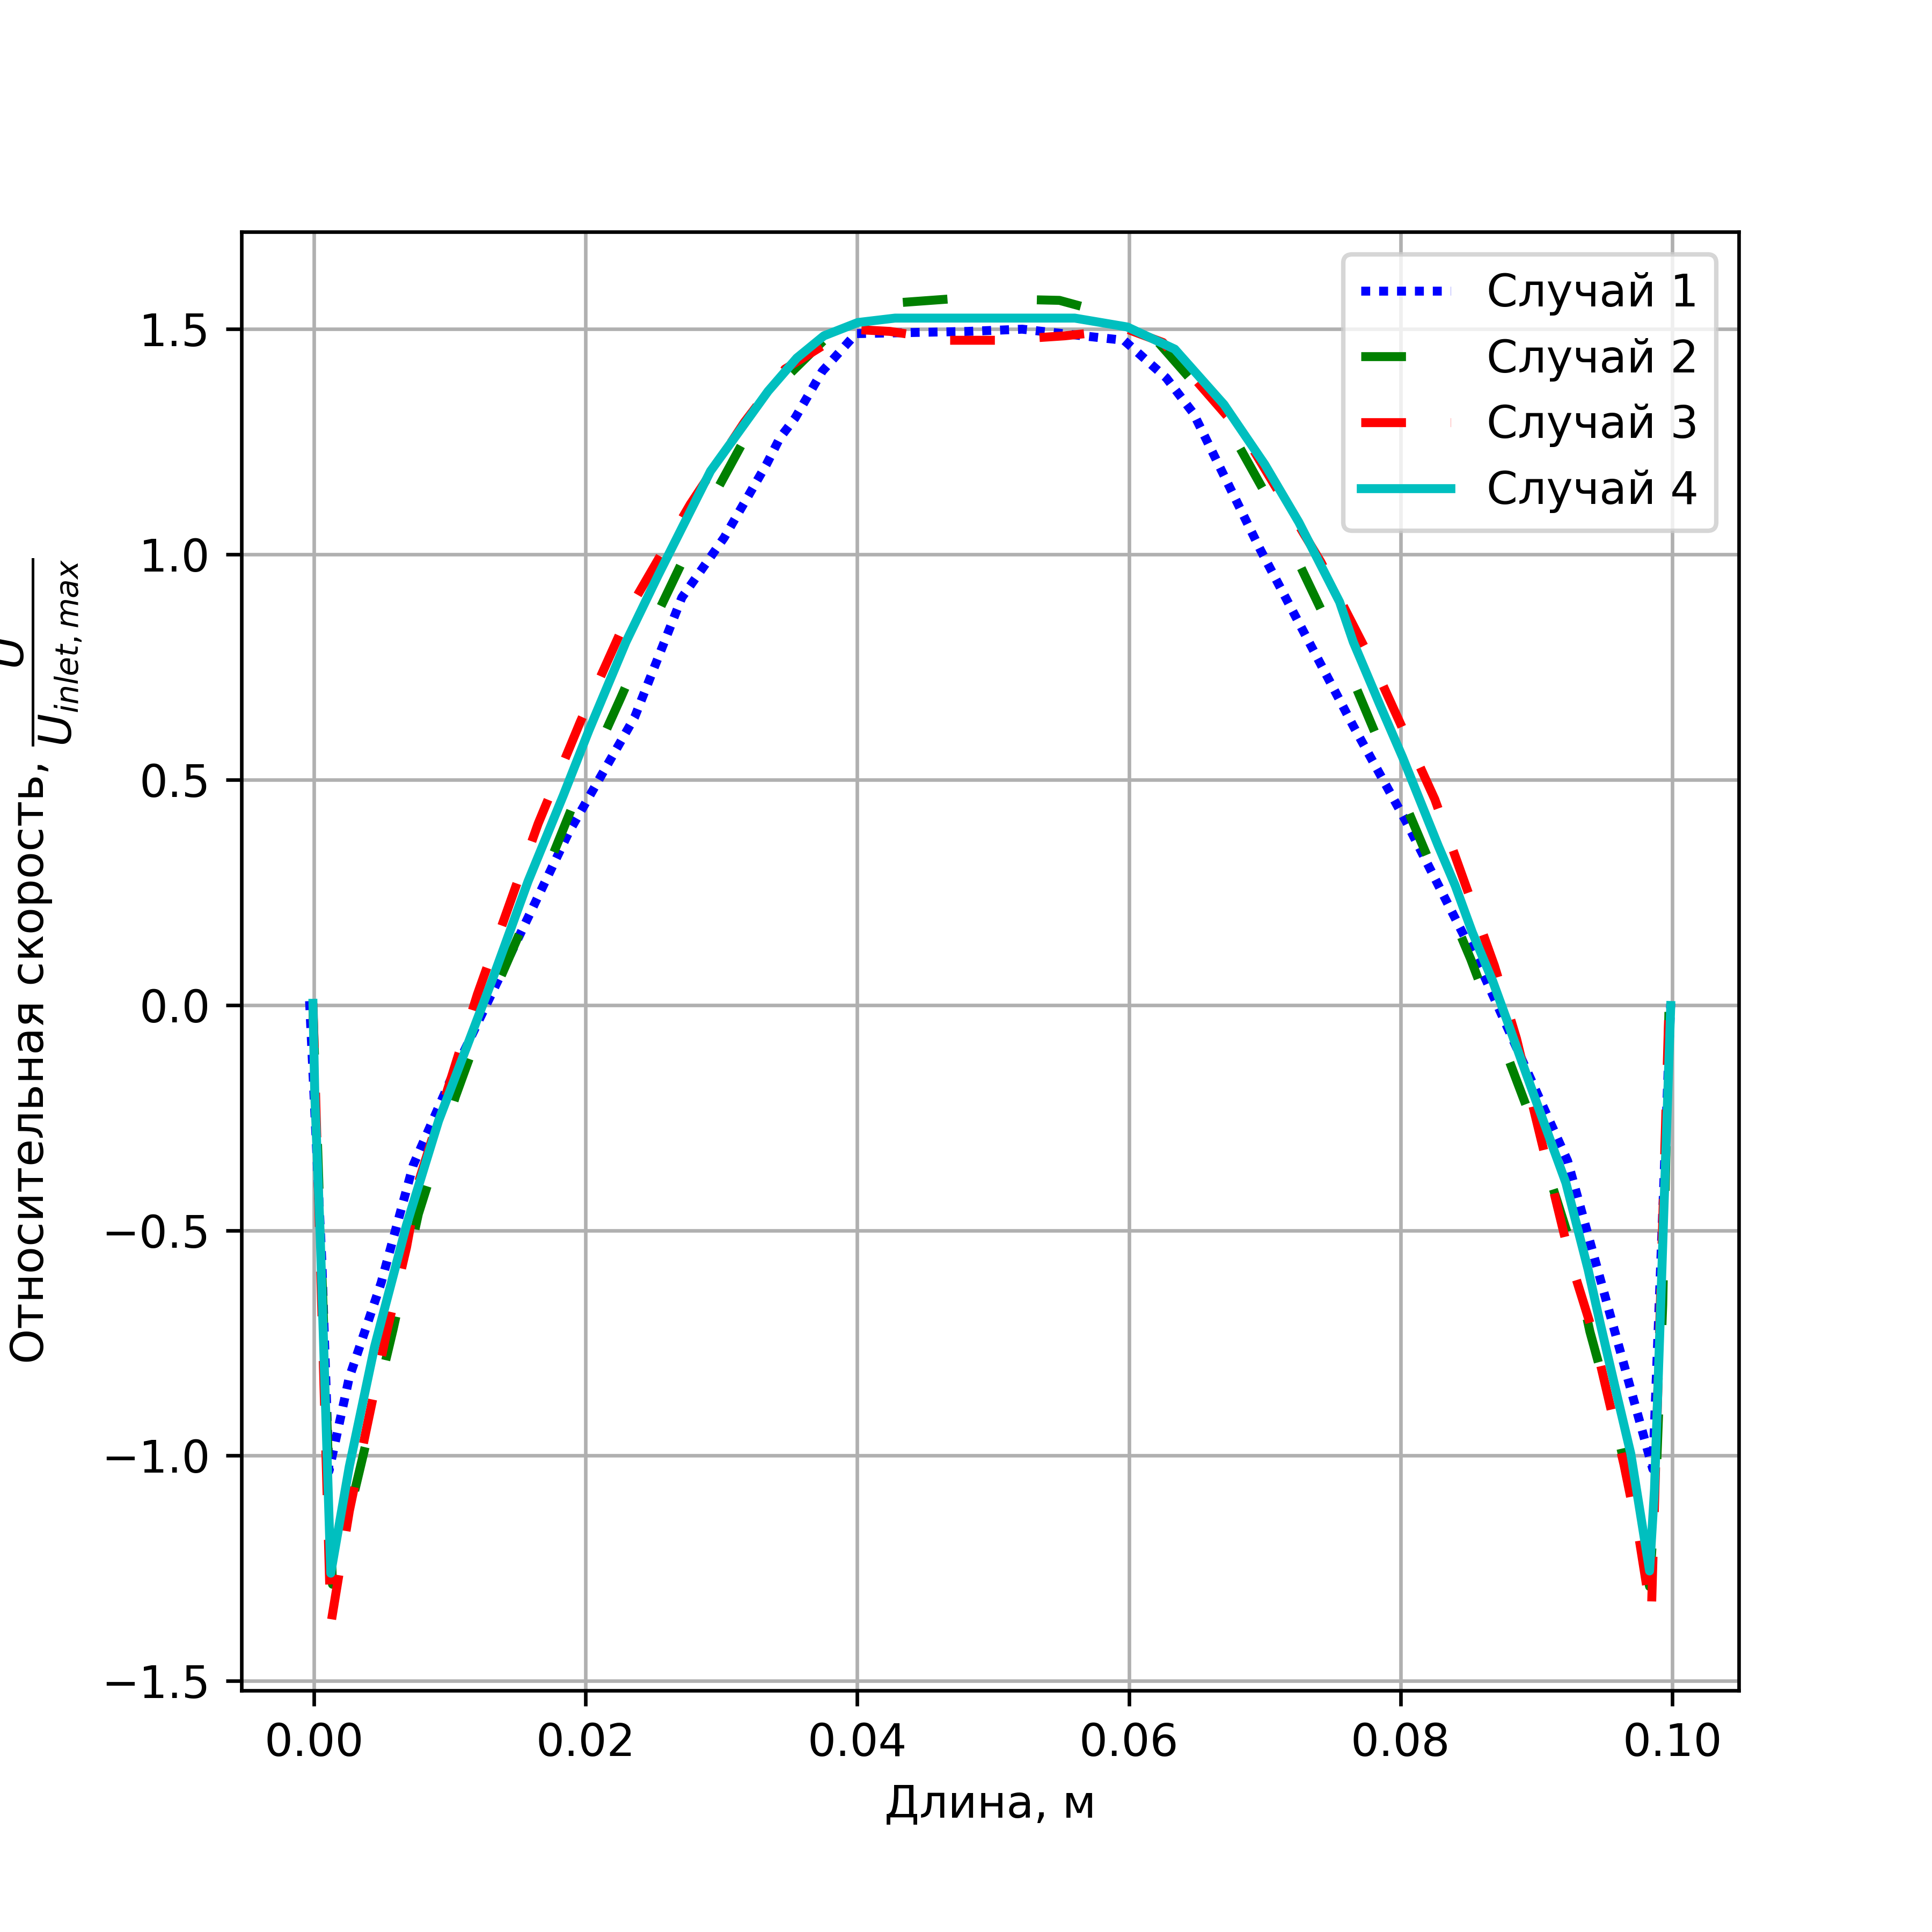
\includegraphics[width=\textwidth]{Synopsis/images/part3/y_velocity_st_20.png}
		\end{subfigure}
		\vfill
		\begin{subfigure}[b]{0.3\textwidth}
			\centering
			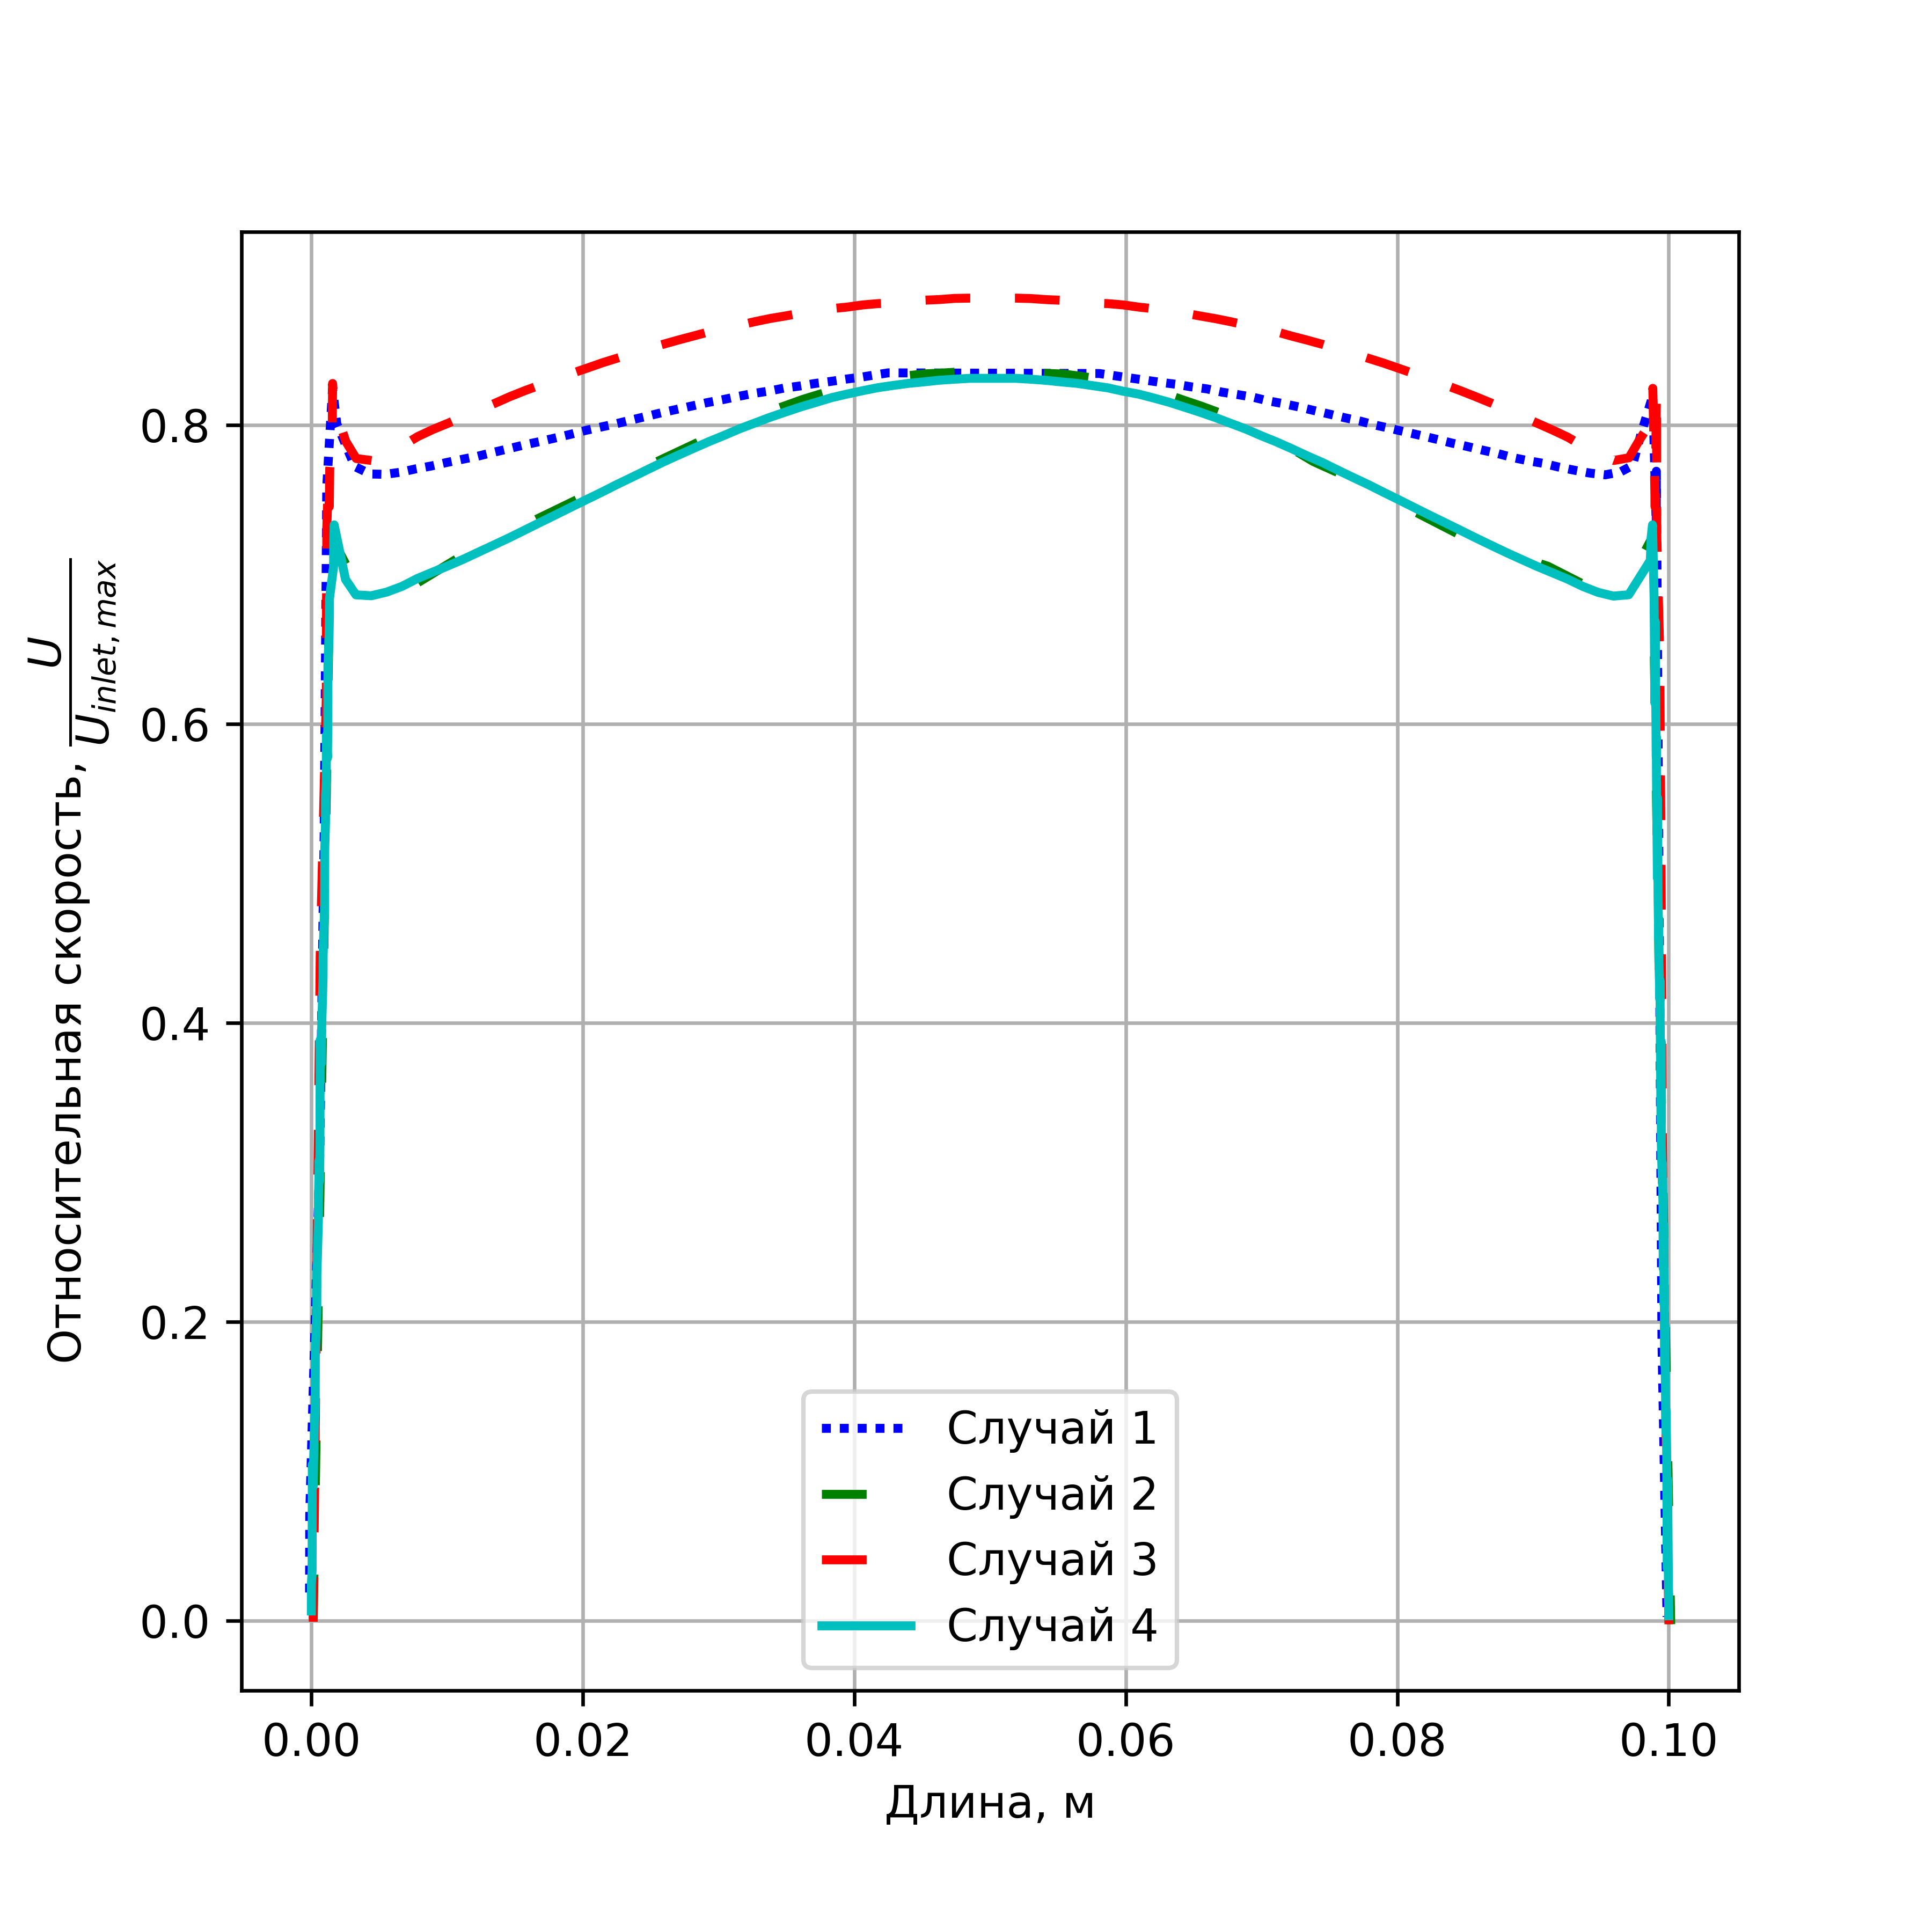
\includegraphics[width=\textwidth]{Synopsis/images/part3/z_velocity_st_1.png}
		\end{subfigure}
		\hfill
		\begin{subfigure}[b]{0.3\textwidth}
			\centering
			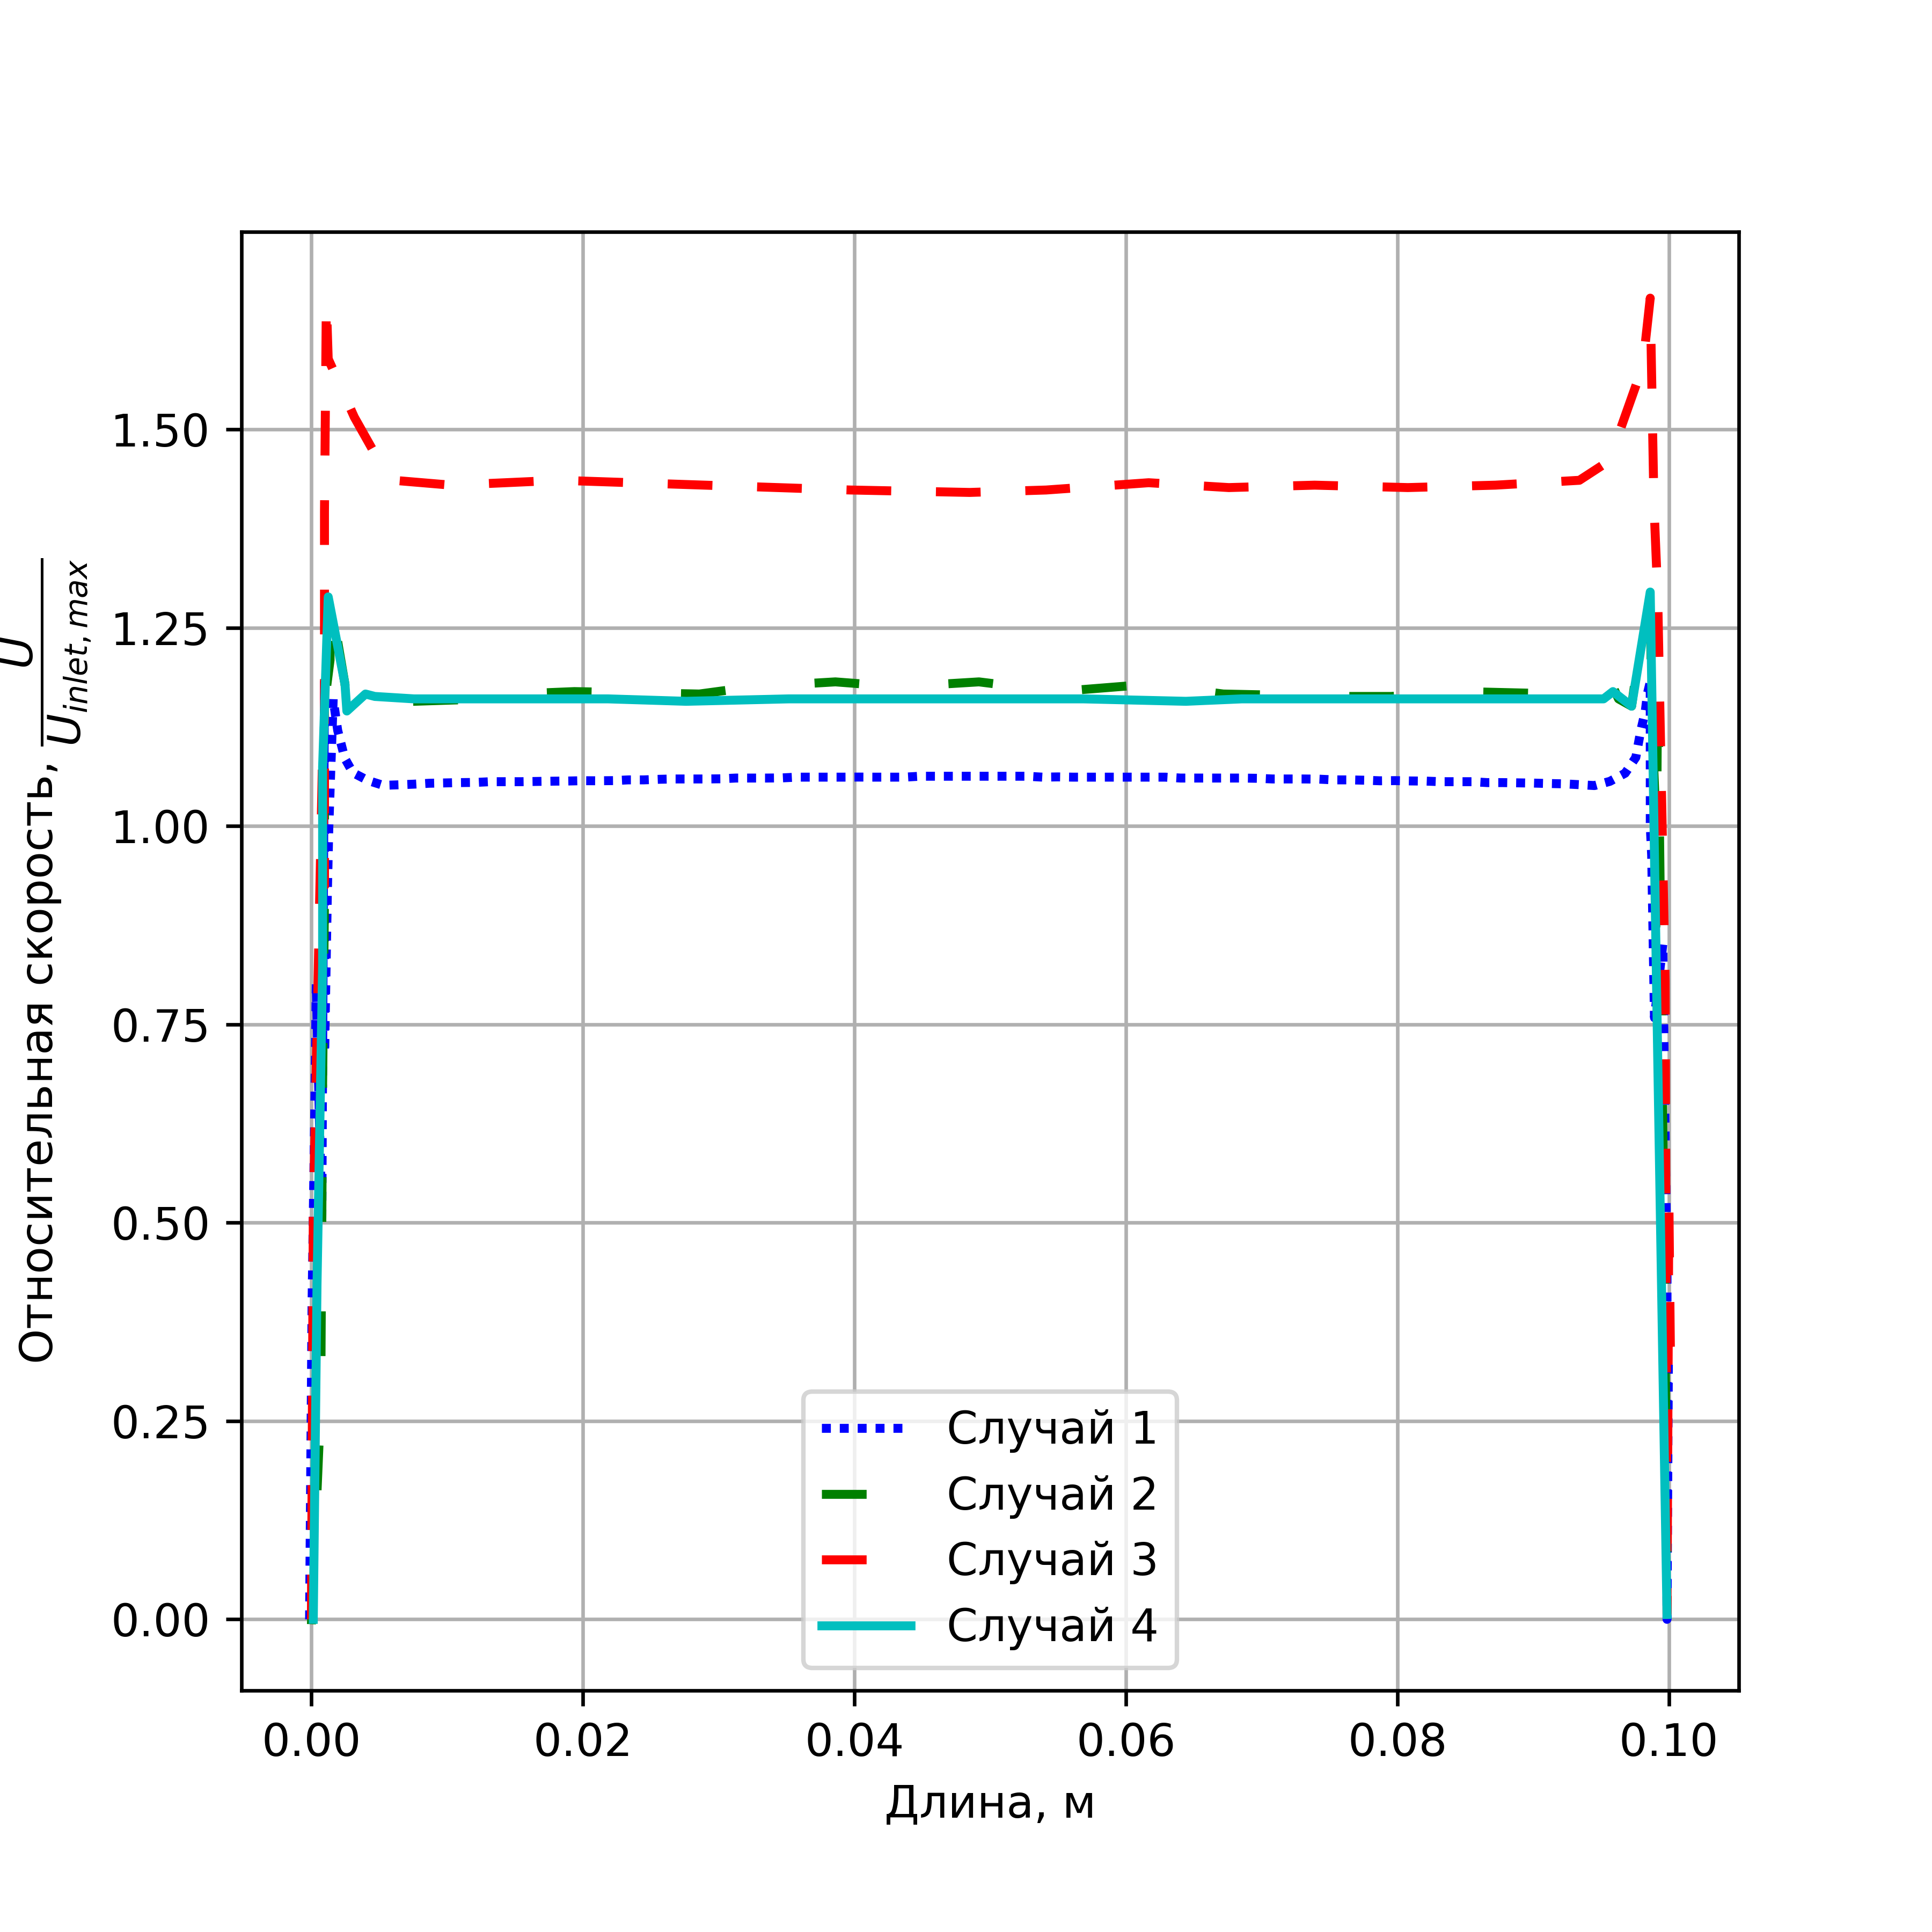
\includegraphics[width=\textwidth]{Synopsis/images/part3/z_velocity_st_5.png}
		\end{subfigure}
		\hfill
		\begin{subfigure}[b]{0.3\textwidth}
			\centering
			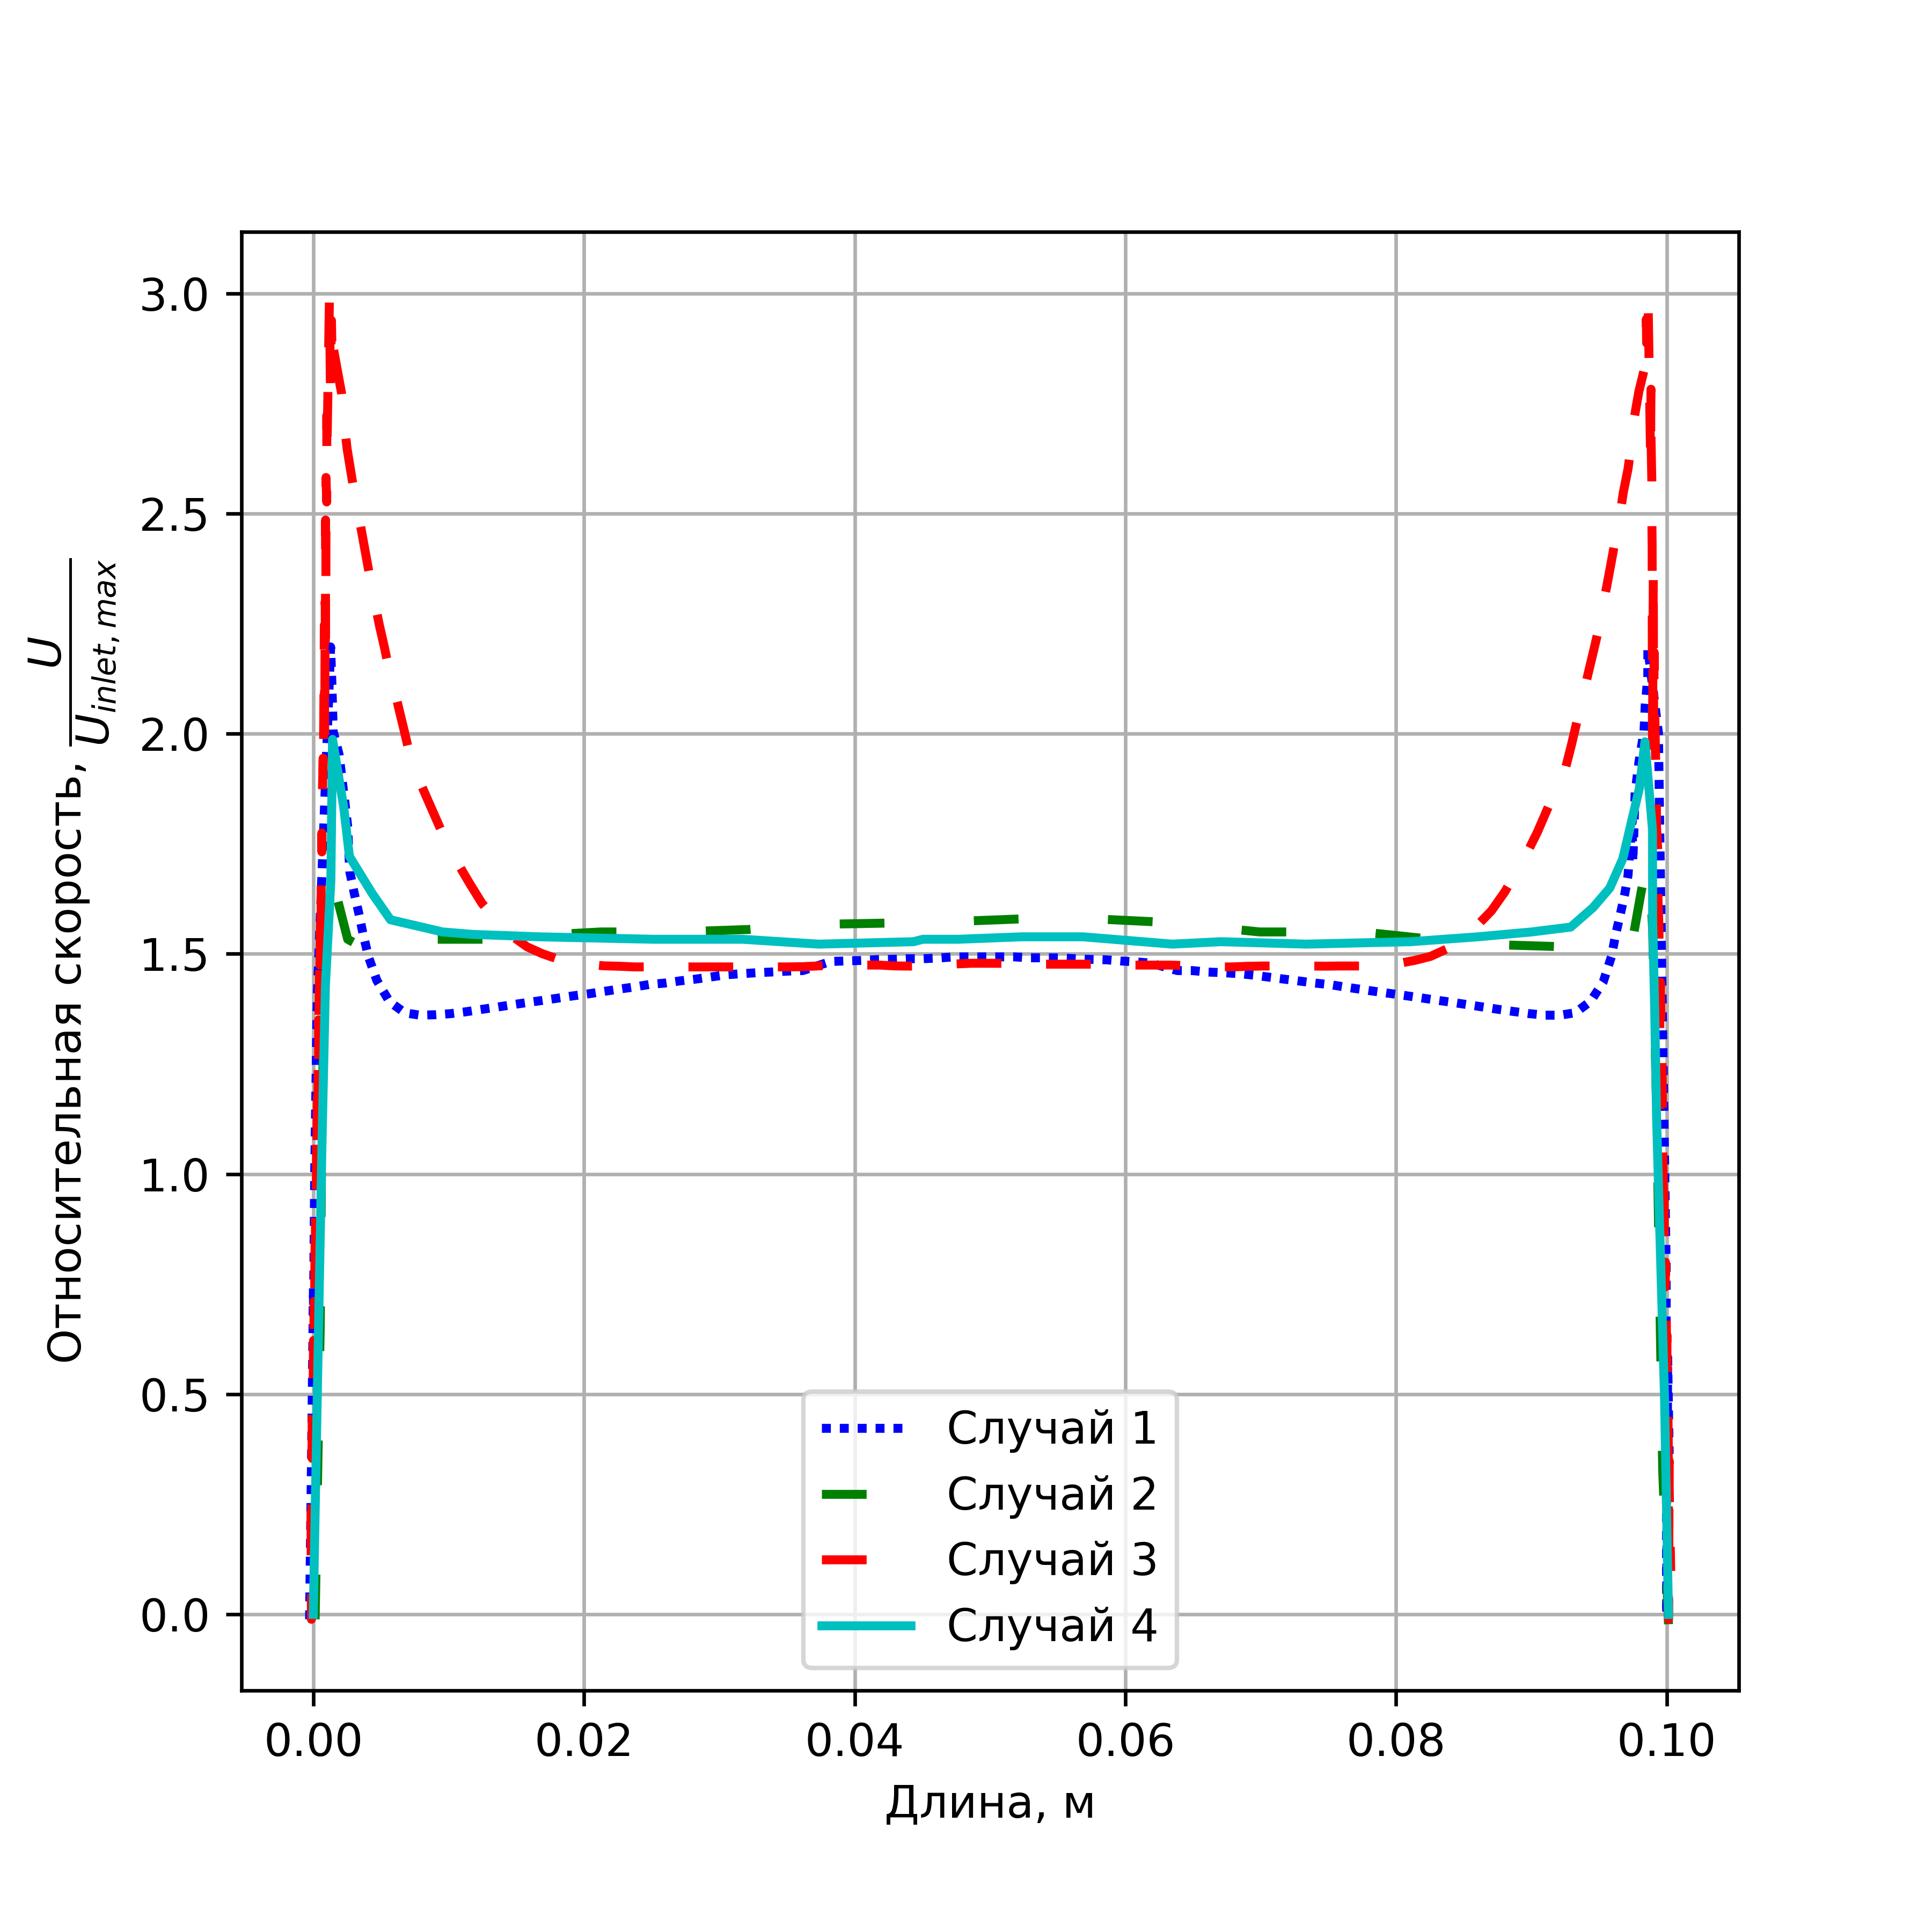
\includegraphics[width=\textwidth]{Synopsis/images/part3/z_velocity_st_20.png}
		\end{subfigure}
		
	}
	\caption{Распределение скорости между стенками перпендикулярными и параллельными магнитному полю для чисел Стюарта а) 1, б) 5, в) 20}
	\label{fig:velocity_cases_comparison}
\end{figure}

Удельная скорость максимальная в случаи 3 (рис.~\ref{fig:velocity_cases_comparison}), когда не учитывается влияние индуцироанных токов на магнитное поле и учитывается поперечный краевой эффект во всем исследуемом диапазоне чисел Стюарда. Обратные потоки формируются так же, как и в случаях идеального эксперимента. Можно наблюдать, что величина обратных течений практически не зависит от краевых эффектов, но зависит от значения числа Стюарда. 
Ускорение потока около гартмоновских стенок и скорость ядра потока существенно зависит от воздействий краевых эффектов и от числа Стюарда. Из этого можно сделать вывод, что магнитные эффекты в большей степени воздействуют на профиль скорости возле стенок перпендикулярных магнитному полю, а обратные потоки у стенок параллельных магнитному полю образуются как следствие изменения профиля у гартмоновских стенок. Также стоит отметить, что результаты в случаи 2 (влияние только ундуцированных токов) и случай 4 (все эффекты учитываются) не значительно расходятся. Из этого можно сделать вывод, о том что наибольший вклад в формировании профиля скоростей вносит продольный краевой эффект. А если сравнить результаты из  случая 3 и случая 1, можно наблюдать, что скорость выше во всем профиле скорсотей с наличием поперечного краевого, чем в случаи идеального магнитного поля. 

Пиковые значения скорости изменяются линейно от числа Стюарда только в диапазоне его малых значений. При больших числах Стюарда эта зависимость становится не линейной и начинает снижать при числах стюрда больше 40, а также прослеживается тенденция к установившемуся значению в середине канала. Этот факт демонстрирует, что существует верхний предел числа Стюарда, когда дальнейшее увеличение магнитной индукции нецелесообразно и не влияет на ускорение в большей части поперечного канала. 

Значительная разница скорости между пиковыми значениями приводит к увеличению градиента давления между этими точками и как следствие к неустойчивым состояниям и возникновению турбулентностей. Возникающая нестабильность течения имеет свой характер, определяемый временем и пространством. На рис~\ref{fig:motion_vortex} линии тока скорости отмечены значениями кинетической энергии в разные моменты времени и значениями плотности магнитного потока бегущего магнитного поля по длине канала. Вихрь потока возникает в области максимальной кинетической энергии и движется в направлении бегущего магнитного поля с той же скоростью. Таким образом, бегущее магнитное поле приводит в движение результирующий турбулентный поток. 

\begin{figure}[h]
	\centerfloat{
		\includegraphics[width=0.9\linewidth]{Synopsis/images/part3/vortexi.png}
	}
	\caption{Движение вихря потока вслед за бегущим полем.}
	\label{fig:motion_vortex}
	
\end{figure}

В случаи с идеализированным магнитным полем возникают два двухмерных вихря на входе активной зоны канала у стенок (см. выделено красным цветом на Рис.~\ref{fig:induced_vortex}) даже при отсутствии существенного влияния продольного краевого эффекта. Эти два вихря затухают со временем за счет движения по направлению скорости потока. Возникновение и затухание носит периодический характер с половиной периода магнитного поля. Также возникают существенные обратные потоки за счет образование двухмерных вихрей у стенок канала. Количество вихрей изменяется со временем от одного до двух. 

\begin{figure}[h]
	\centerfloat{
	\includegraphics[width=0.9\linewidth]{Synopsis/images/part3/velocity.png}
	}
	\caption{Формирование вихрей в идеализированном случаи.}
	\label{fig:induced_vortex}
\end{figure}
 
На основе полученных результатов влияния магнитных эффектов на потоки жидкости были построены напорно-расходные характеристики насоса для различных чисел подобия (Рис.~\ref{fig:pq_magnetic}). При увеличении магнитного числа Рейнольдса характеристика становиться S-образной так как при малых его значениях стремится к прямой линии. Это утверждение справедливо и в классической теории электромеханики если принять аналогию магнитного числа Рейнольдса с добротностью. Вид гидродинамической внешней нагрузки влияет на магнитные усилия и важно правильно описывать систему при проектировании таких установок. Также для этих характеристик были проанализированы картины поля скоростей на основе которых посроена карта состояний потока для разных чисел подобия (см. Рис.~\ref{fig:map_instability})
\begin{figure}[t]
	\centerfloat{
		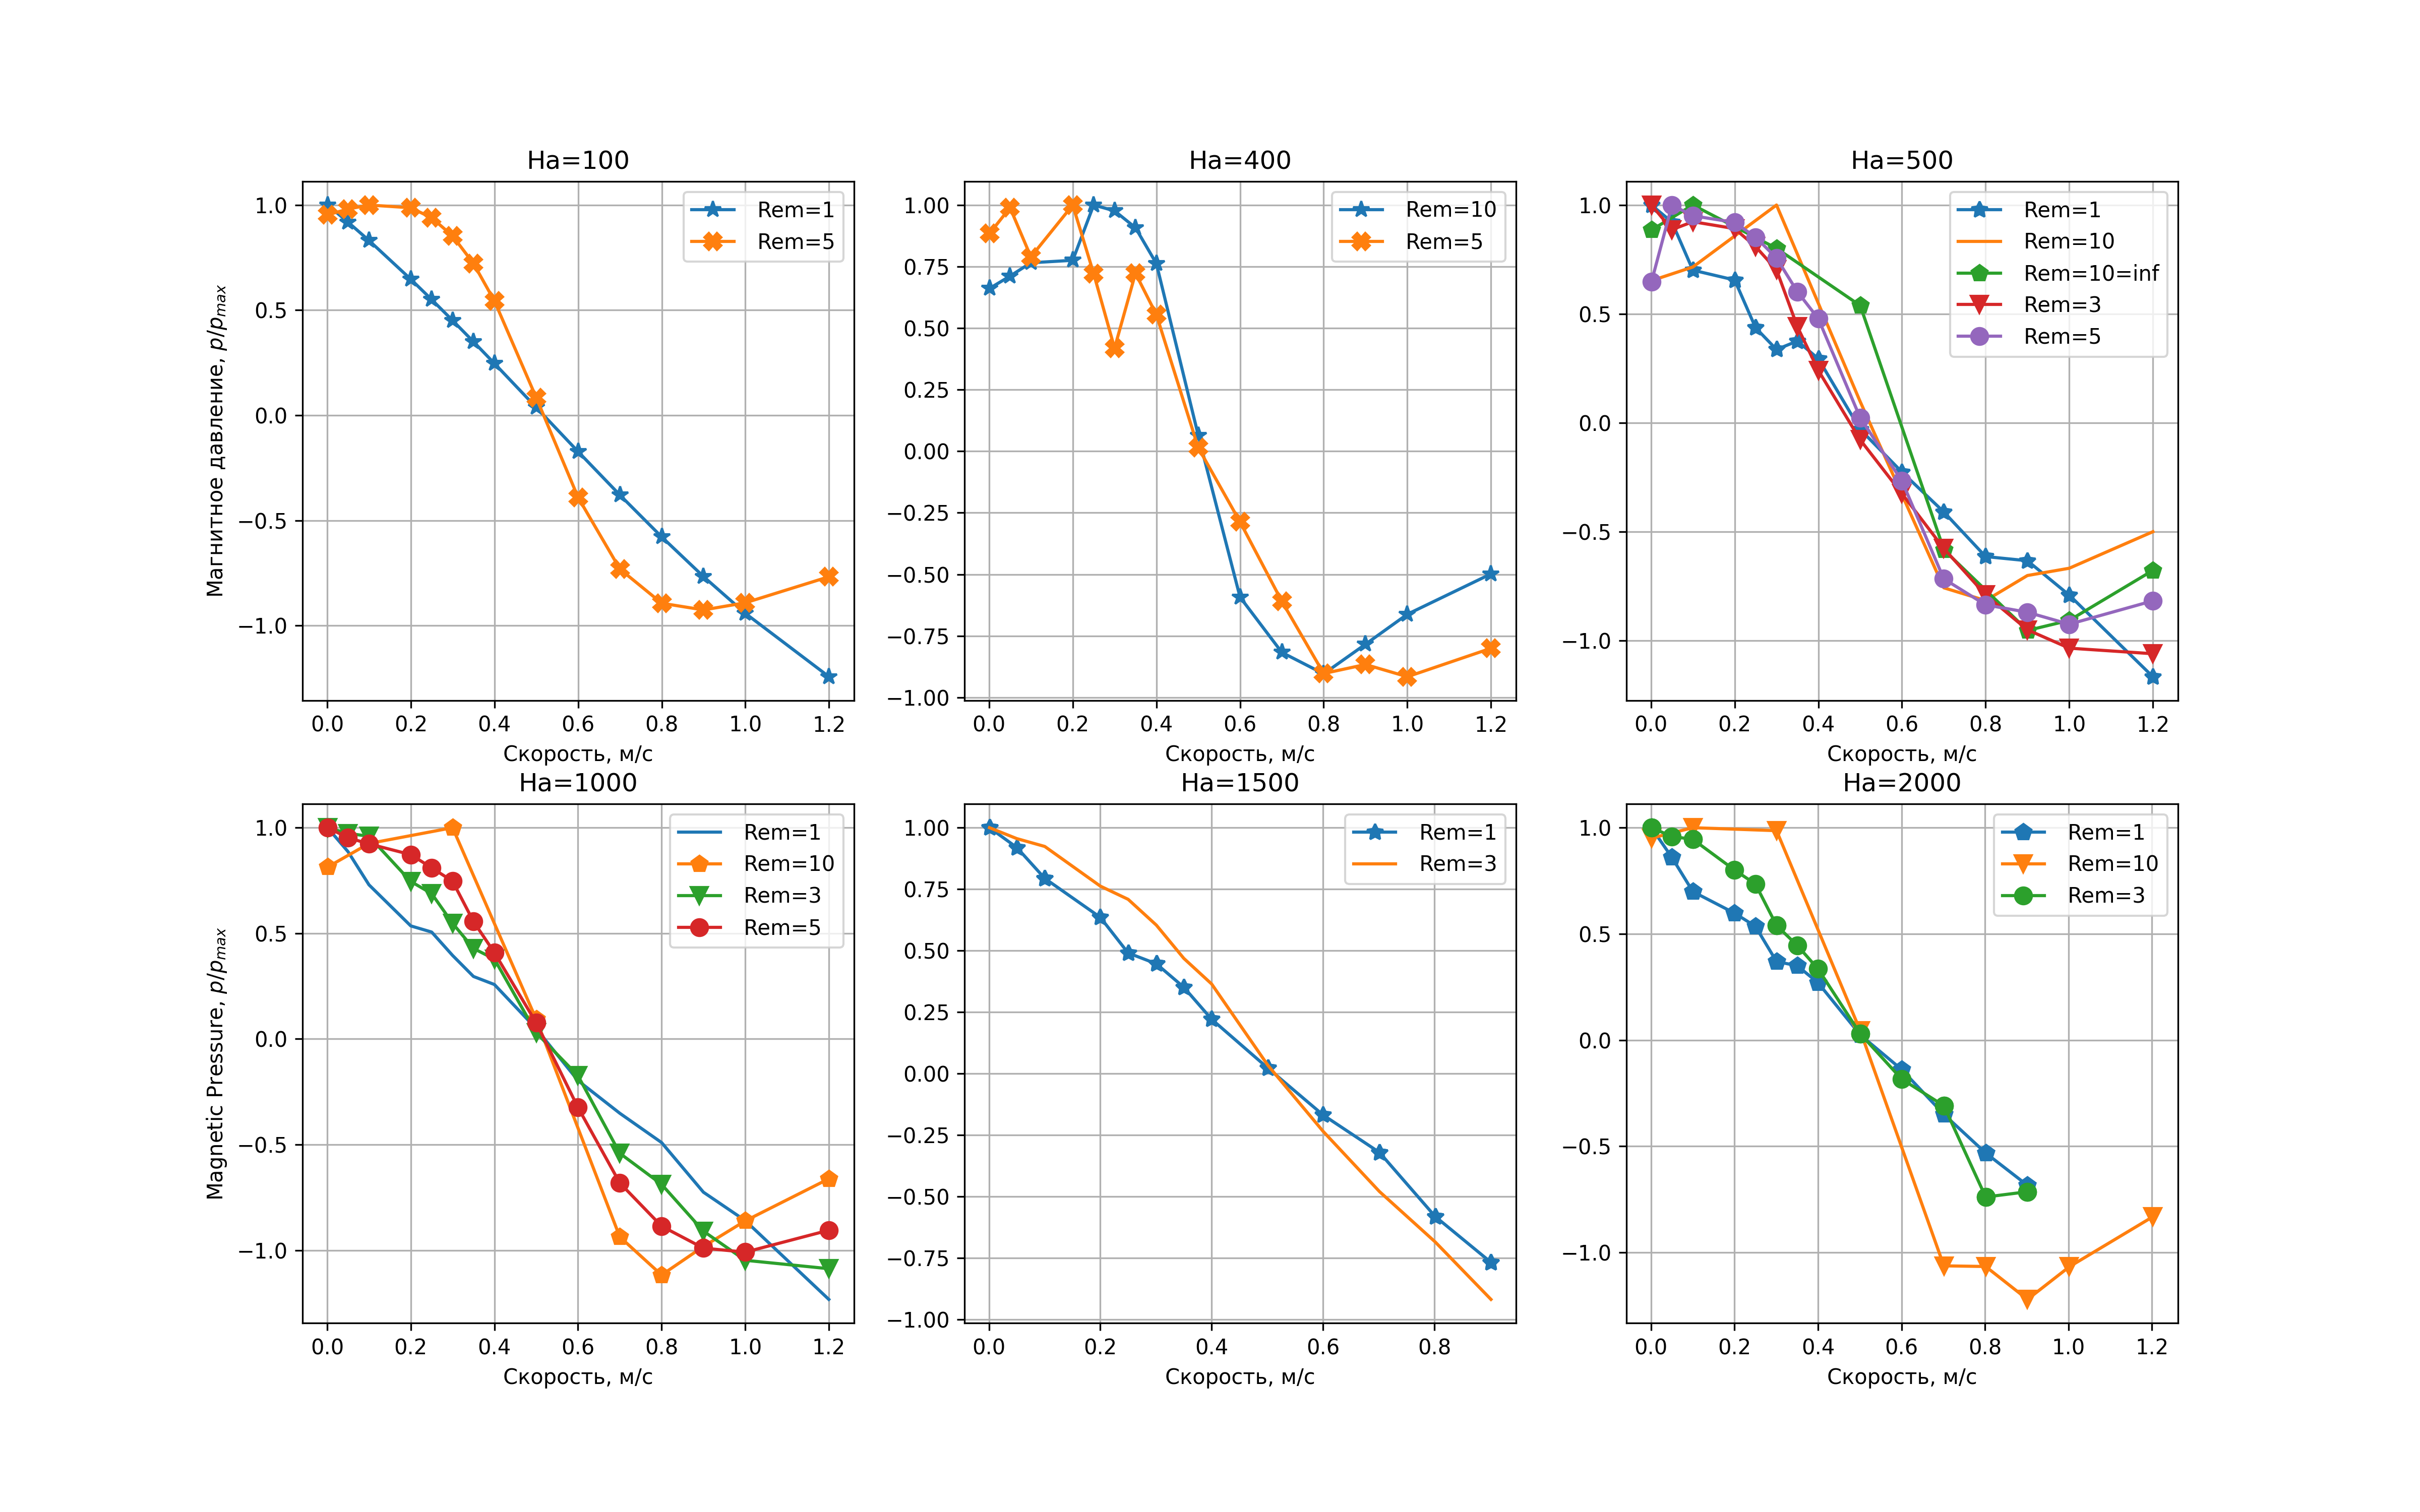
\includegraphics[width=1\linewidth]{Synopsis/images/part3/Magnetic pressure_ru.png}
	}
	\caption{Магнитное давление в зависимости от расхода жидкости.}
	\label{fig:pq_magnetic}
\end{figure}

Турбулентные течения характеризиуются большой кинитческой энергией, которая может разрушать футеровку канала, вызывать сильные механические пульсации метала, мешать протеканию жидкости через сечение канала и приводить к ряду других нежелательных явлений. Одним из механизмов появления обратных течений является закон сохранения массы $div \mathbf{U} = 0$, который описывает, что среднее значение через заданное сечение должно быть равно постоянному числу. Следовательно, если локально в сечении происходит увеличении скорости, в другом месте должна быть просадка скорости для сохранения постоянной средней скорости в сечении канала. Эти результаты могут быть использованы в проектировании индукционных насосов при решении проблемы неустойчивости системы и устранения обратных потоков. 

\begin{figure}[h]
	\centerfloat{
		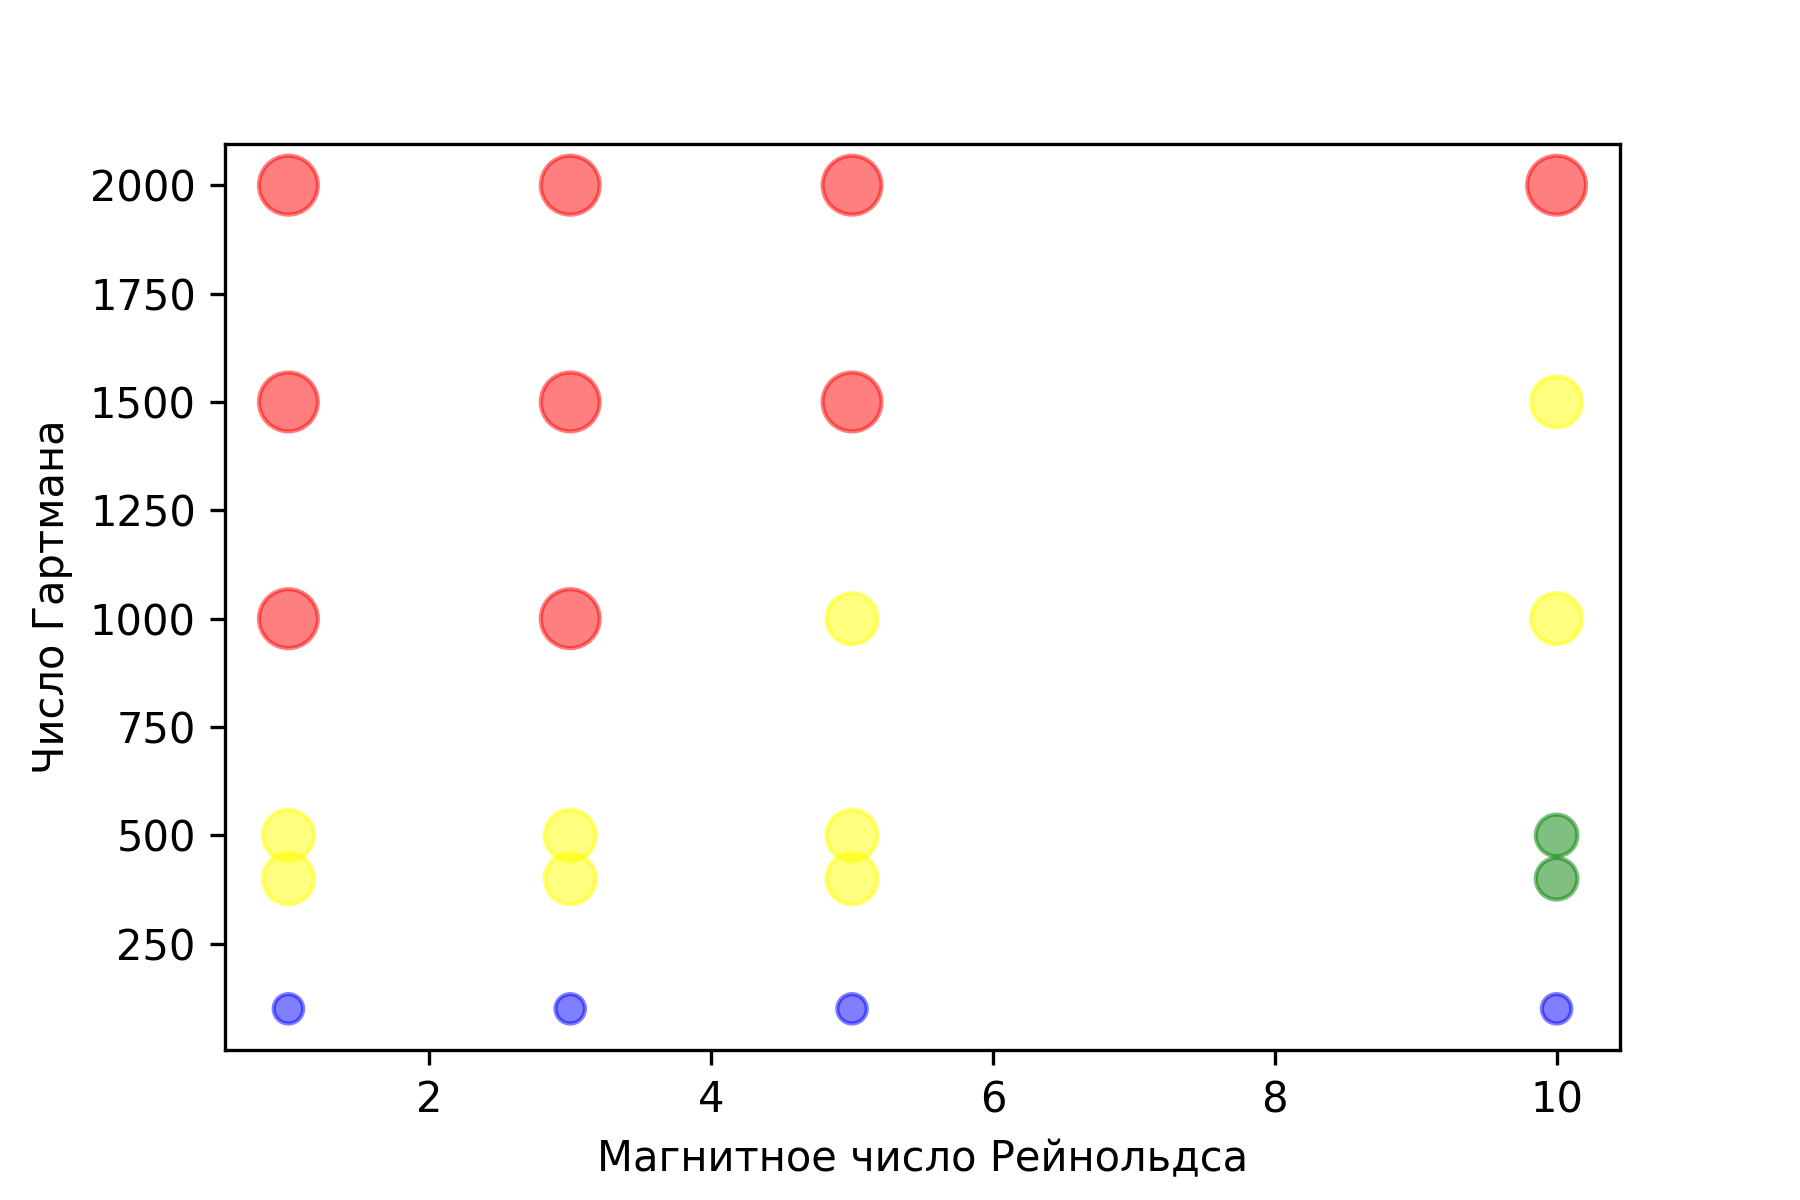
\includegraphics[width=0.5\linewidth]{Synopsis/images/part3/map_vortex_2d.png}
	}
	\caption{Картина возникновения вихрей. Синий цвет -- устойчивое ламинарное состояние, зеленый -- локальные возмущения, желтый -- локальные устойчивые вихри, красный -- сильная неустойчивость.}
	\label{fig:map_instability}
\end{figure}


В \underline{\textbf{четвертой главе}} проведен анализ влияния тепловых процессов на поведение потока жидкости в прямоугольном канале с аспектным соотношением ширины и высоты равным 2. Постановка задачи аналогичная описанной в третьей части этой работы с добавлением граничных условий для температуры. Задается постоянная разность температур между стенками перпендикулярными магнитному полю, а остальные стенки рассматриваются как теплоизолированные. На Рис.~\ref{fig:heat_velocity} показаны распределения скорости вдоль линии в центре канала между стенками пермендикулярными (а) и параллельными (б) магнитному полю для разницы 0, 10 и 30 температур между стенками без воздействия на канал магнитного поля, с воздейсвтием магнитного поля, но без учета тепловыделения и с учетом тепловыделения. Эти результаты рассчитаны для числа Гартмана 100, магнитного Рейнольдса 10, гидродинамического числа Рейнольдса 10000 и числа Стюарта 1. Помимо распределения скорости в работе построены температурные картины. Разница между результатами с учетом источника нагрева и без составляет около 5~\%, а для распределения температур не превыше 0.01~\%, но даже это не значительное изменение приводит к значительным колебаниям скорости потока жидкости. Большее влияние на распределение температур вносит наличие массо переноса из-за лоренцевских сил. Чем выше разница температур между стенками, тем сильнее влияние джоулева тепла на скорость потока. 

\begin{figure}[h]
	\centering{
		\begin{subfigure}[b]{0.48\textwidth}
			\centering
			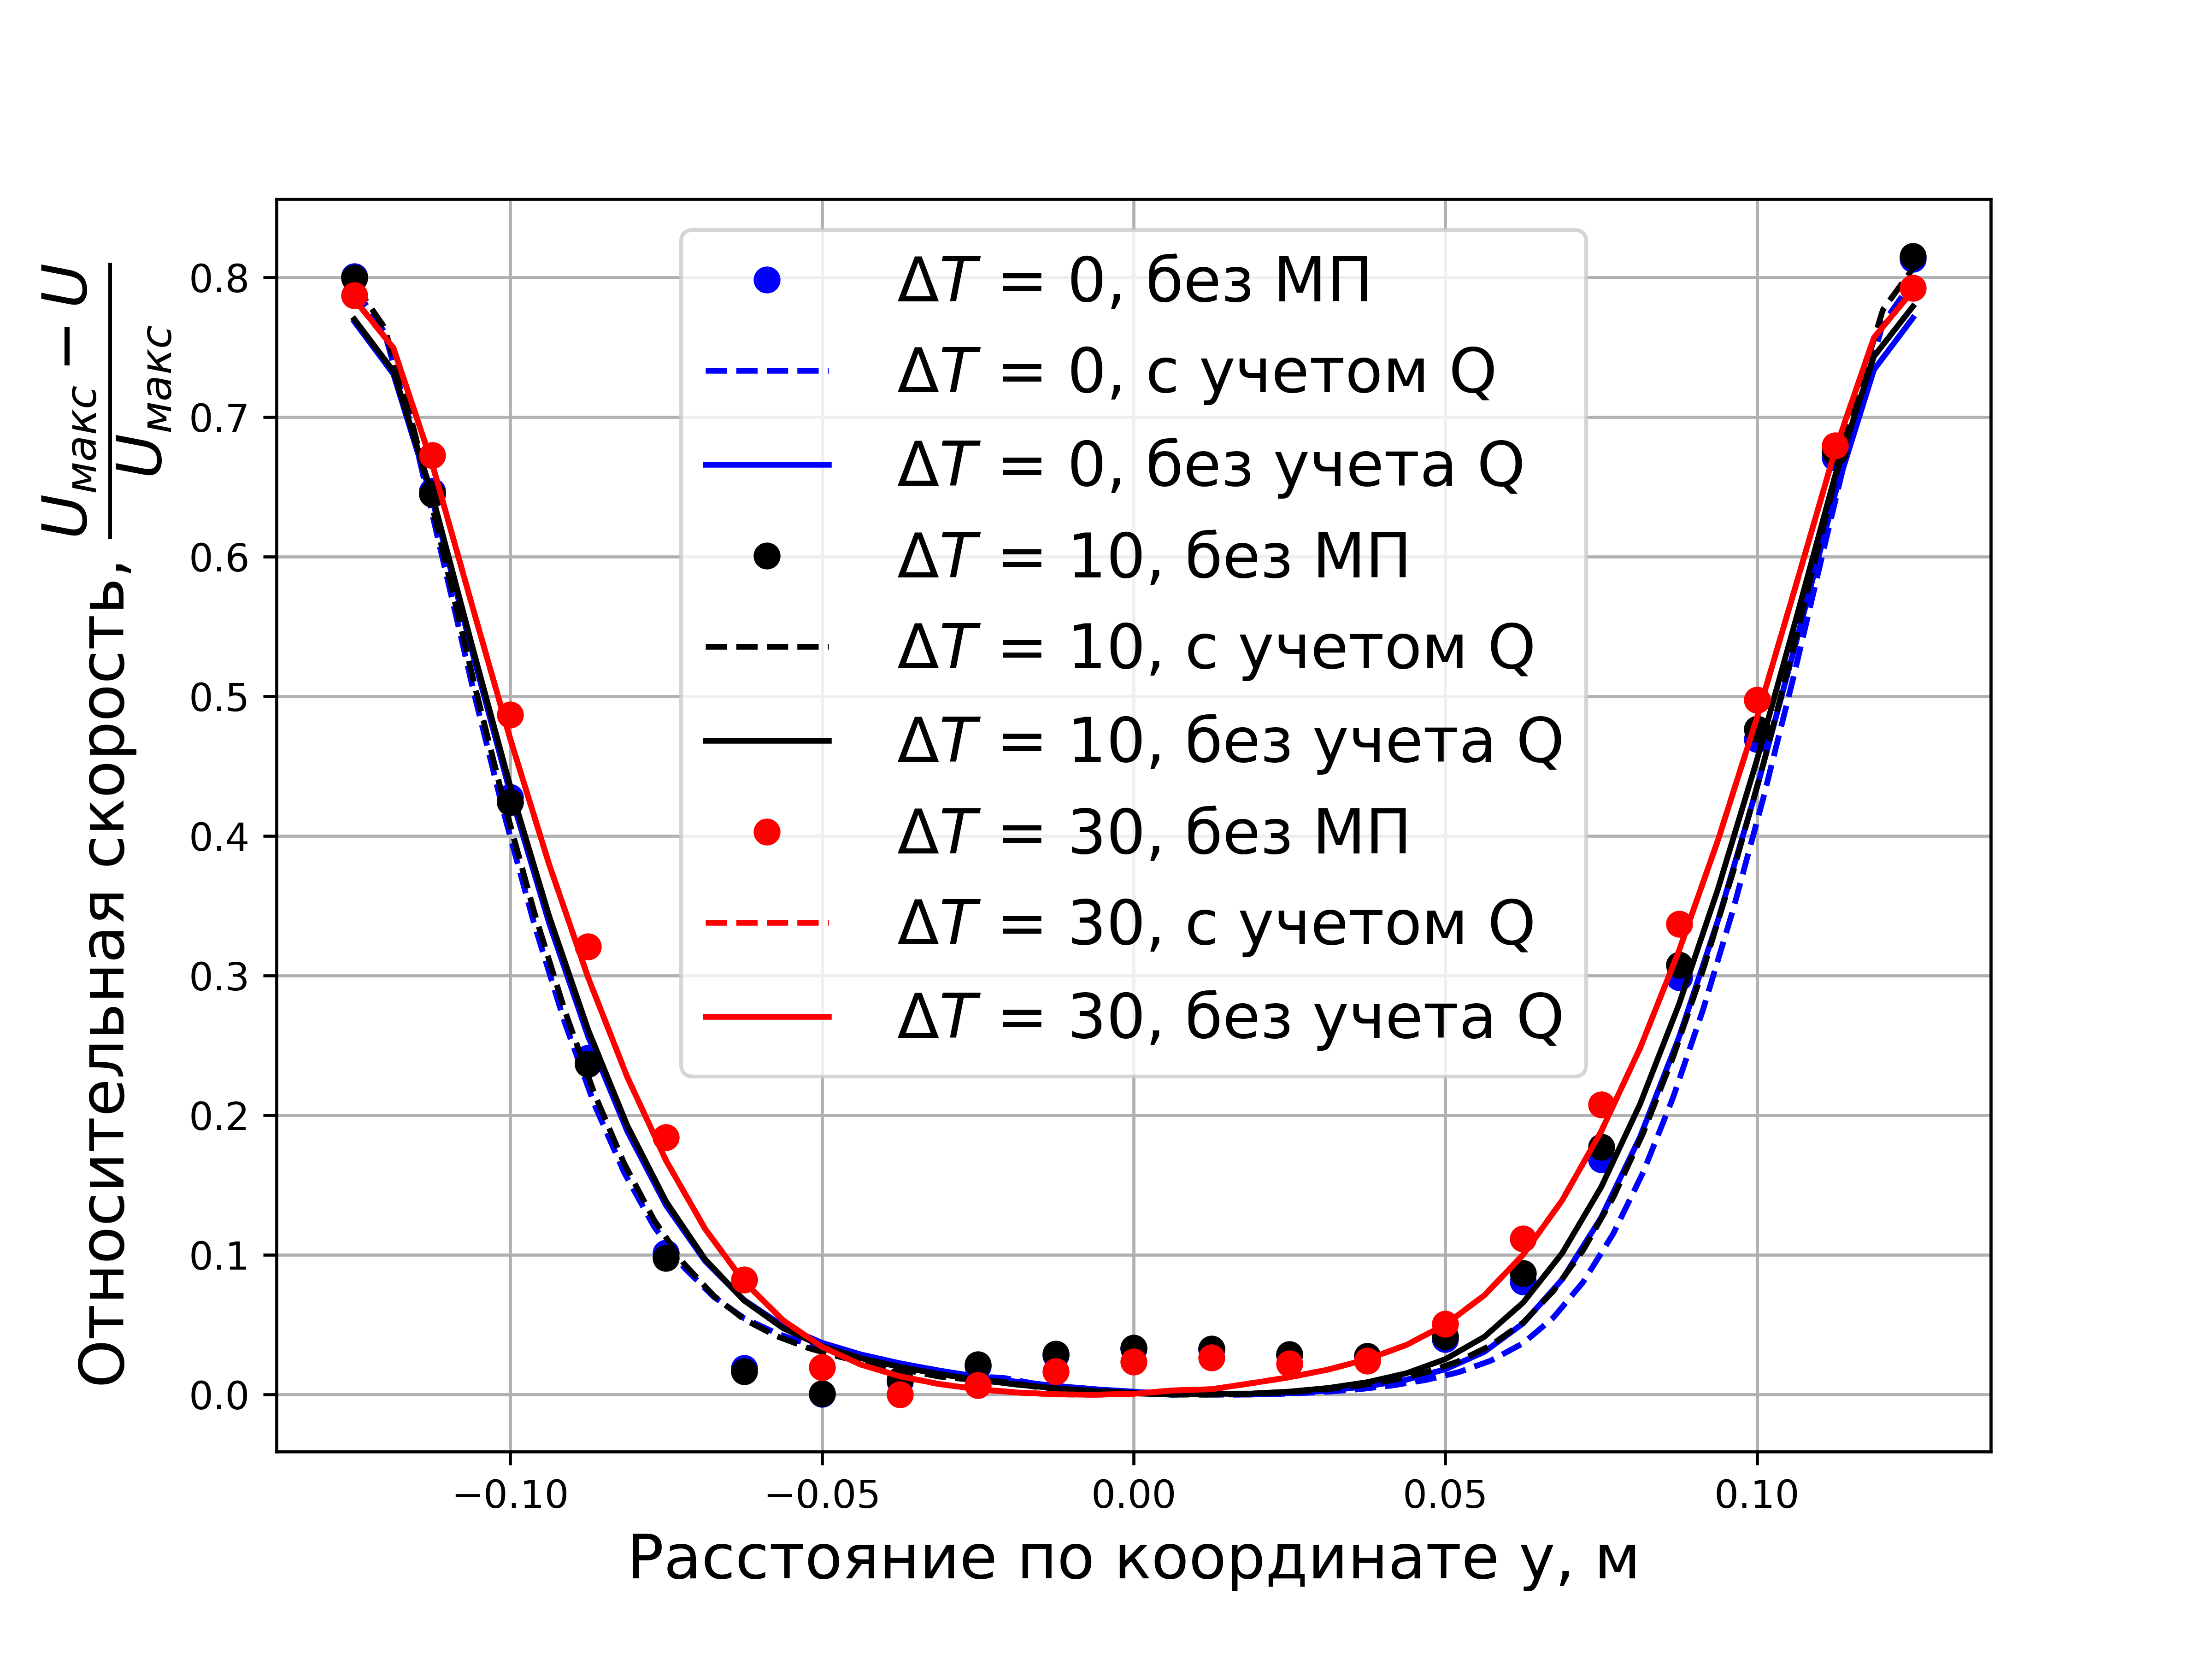
\includegraphics[width=\textwidth]{Synopsis/images/part4/y_Velocity_ru.png}
		\end{subfigure}
		\hfill
		\begin{subfigure}[b]{0.48\textwidth}
			\centering
			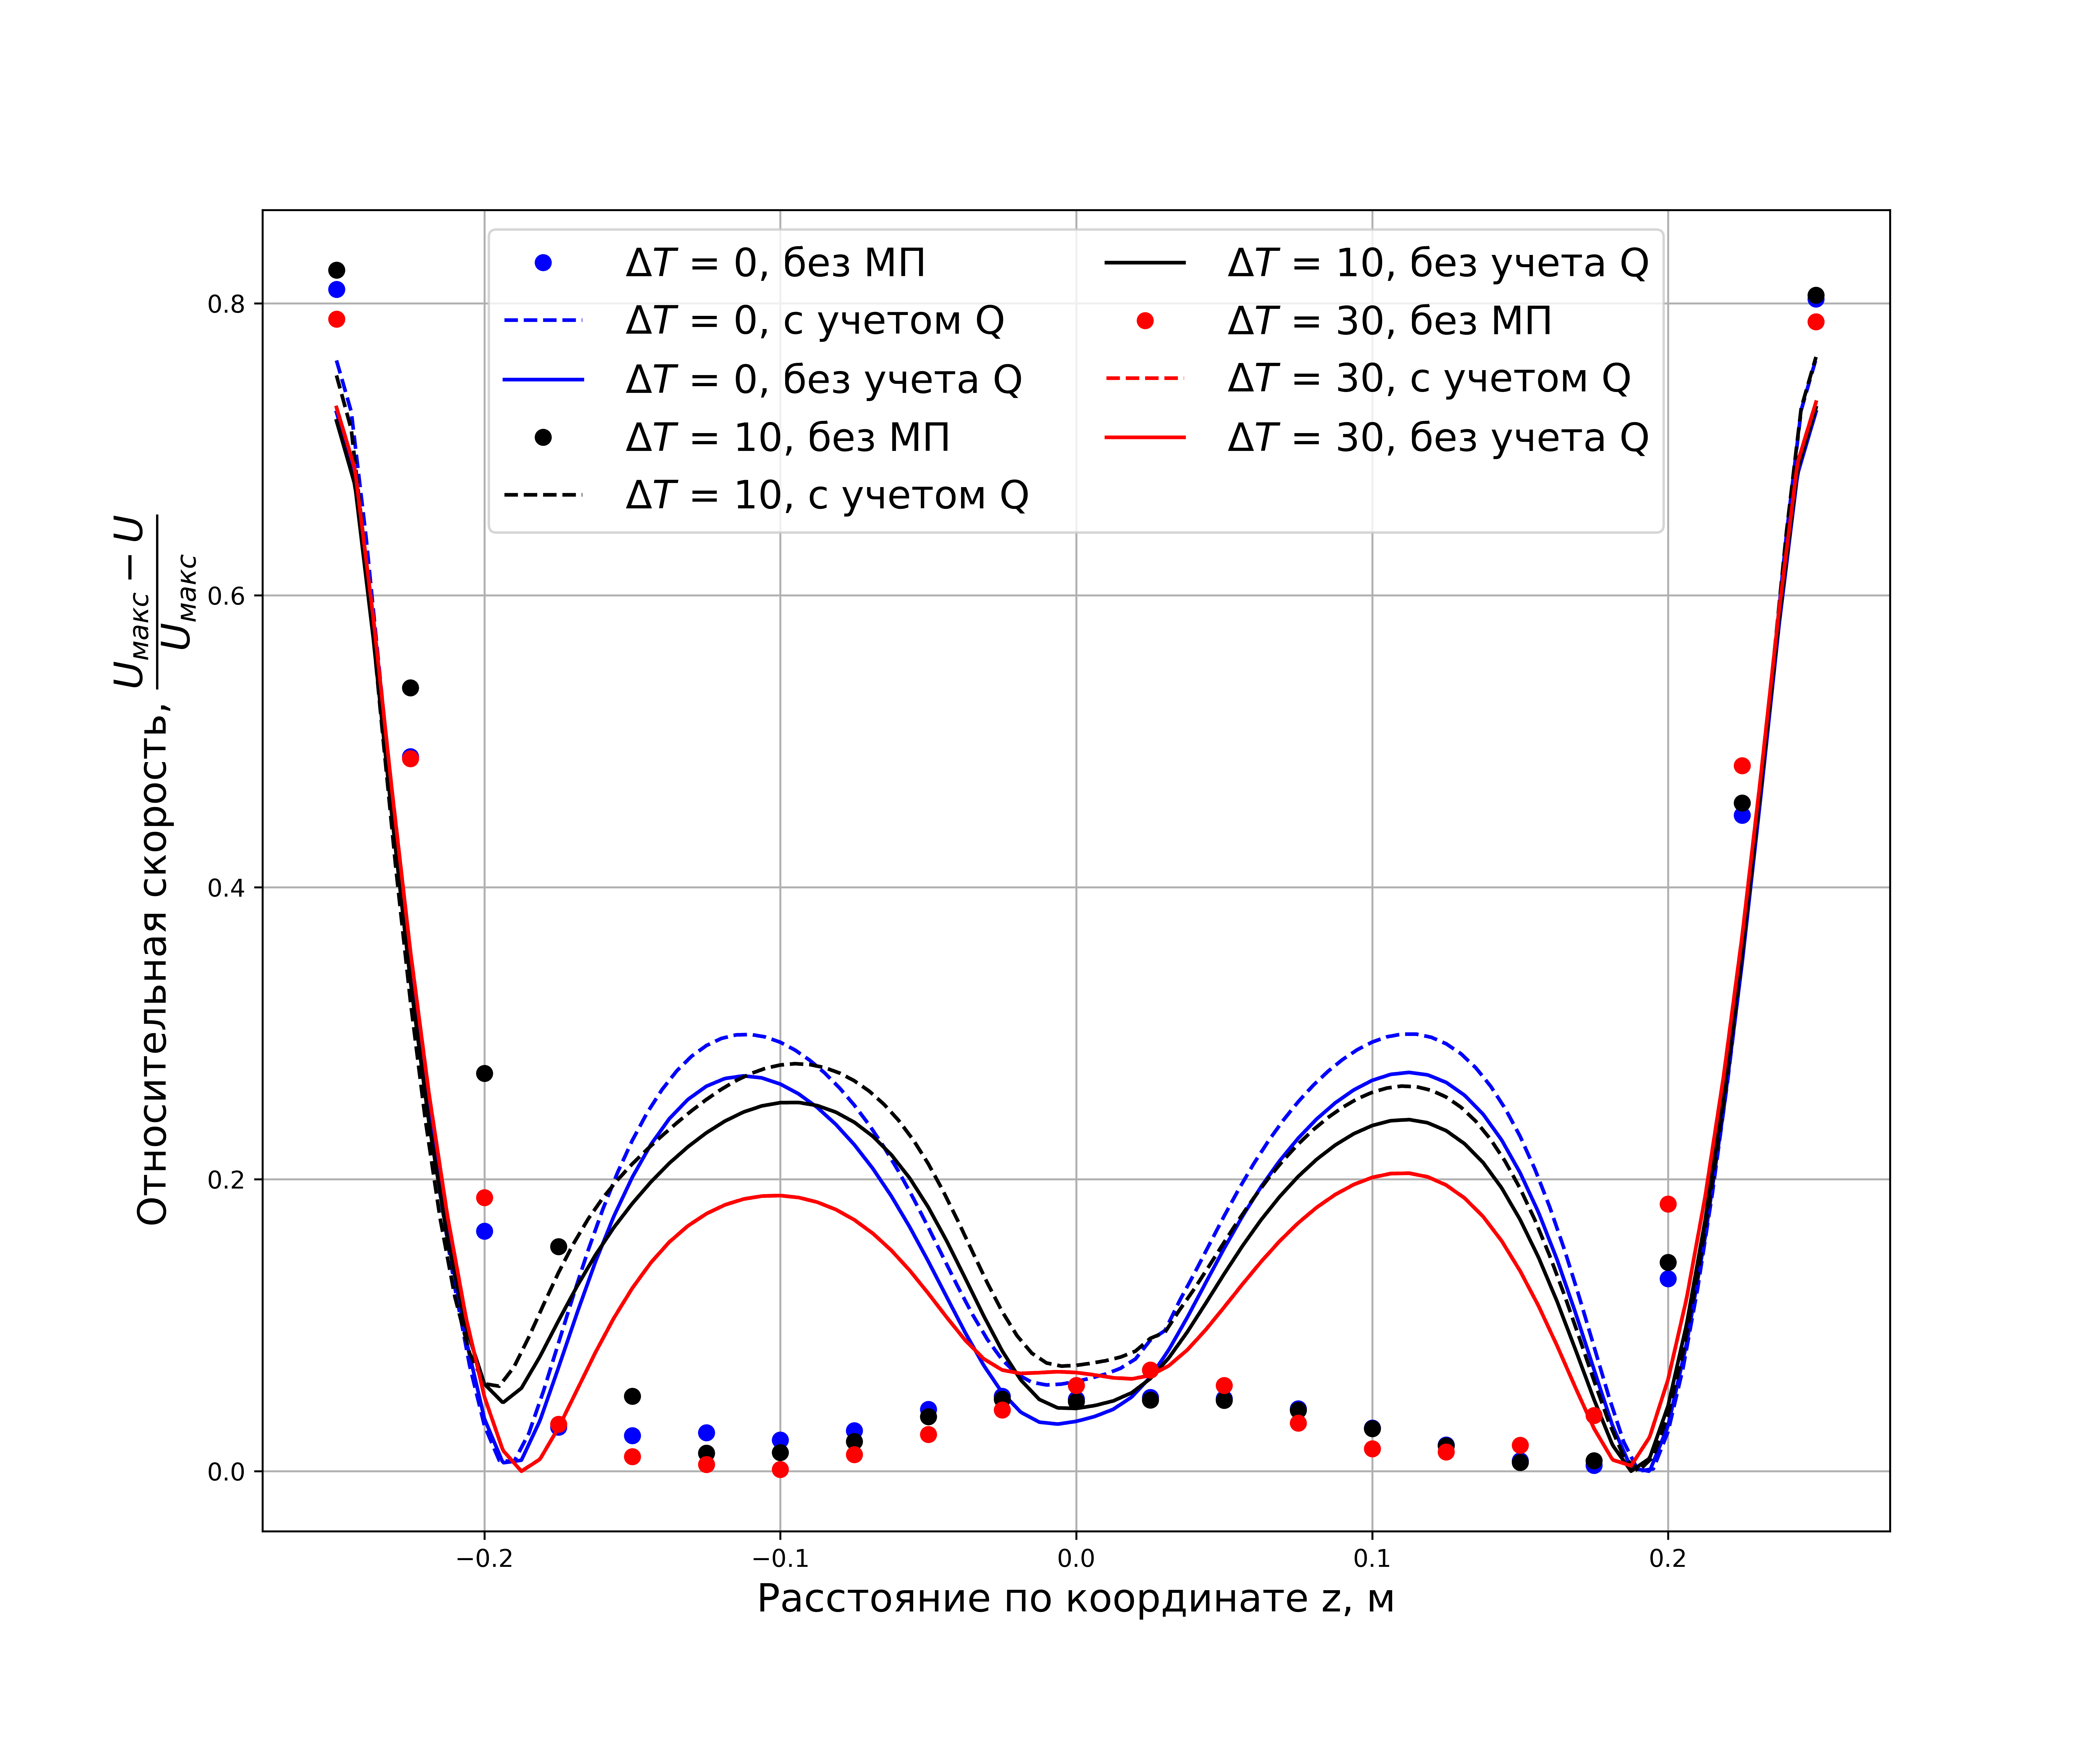
\includegraphics[width=\textwidth]{Synopsis/images/part4/z_Velocity_ru.png}
		\end{subfigure}
	}
	\caption{Относительная скорость между стенками (а) перпендикулярными и (б) параллельными магнитному полю с различными значениями разницы температур между перпендикулярными стенками}
	\label{fig:heat_velocity}
\end{figure}

Важность этого исследования объясняется значительными градиентами температуры входной жидкости (в металлургии при разливки магния разница темпераутр достигает 100 C\si{\degree}) низким КПД (менее 20~\%) электромагнитных насосов, как следсвие высоким тепловыделением. В последующих работах интерес выывает подобные исследования для низкций чисел магнитного Рейнольдса и высоких значениях Гартмана, также учет числа Прандтля и неравномерности магнитного поля из-за особеннойстей конструкций катушек. 


В \underline{\textbf{пятой главе}} проведены исследования по чувствительности сетки и модели турбулентности на точность результатов. Даются рекоммендации по выбору модели турбулентности для оптимального соотношения между временем расчета и точностью результатов. Также обсуждается процедуры разделения уравнения момента на уравнения для давления и скорости используя PIMPLE и PISO циклы для их решения. Рассматривается возможность снижения количества уравнений за счет корректной настройки сетки. 


\FloatBarrier
\pdfbookmark{Заключение}{conclusion}                                  % Закладка pdf
В \underline{\textbf{заключении}} приведены основные результаты работы, которые заключаются в следующем:
%% Согласно ГОСТ Р 7.0.11-2011:
%% 5.3.3 В заключении диссертации излагают итоги выполненного исследования, рекомендации, перспективы дальнейшей разработки темы.
%% 9.2.3 В заключении автореферата диссертации излагают итоги данного исследования, рекомендации и перспективы дальнейшей разработки темы.
\begin{enumerate}
  \item На основе анализа неустойчивых состояний было показано важность учета трехмерных моделей и адекватный выбор моделей турбулентности для расчета потоков жидкости в каналах, находящийся под воздействием магнитного поля. 
  \item Численные исследования показали, что температурное поле влияет на распределение скорости при определенных значениях числа Прандтля. Краевые эффекты магнитного поля вносят не только отрицательное действие, но в ряде случаев могут улучшить поведение потока. 
  \item Для выполнения поставленных задач был созданы процедуры решения связанных мультидисциплинарных задач на основе программ с открытым кодом. Для упрощения процедуры расчетов был написан код с опциями автоматической настройки моделей, сетки, обработки результатов и ряда других возможностей. 
\end{enumerate}


\pdfbookmark{Литература}{bibliography}                                % Закладка pdf

\ifdefmacro{\microtypesetup}{\microtypesetup{protrusion=false}}{} % не рекомендуется применять пакет микротипографики к автоматически генерируемому списку литературы
\urlstyle{rm}                               % ссылки URL обычным шрифтом
\ifnumequal{\value{bibliosel}}{0}{% Встроенная реализация с загрузкой файла через движок bibtex8
    \renewcommand{\bibname}{\large \bibtitleauthor}
    \nocite{*}
    \insertbiblioauthor           % Подключаем Bib-базы
    %\insertbiblioexternal   % !!! bibtex не умеет работать с несколькими библиографиями !!!
}{% Реализация пакетом biblatex через движок biber
    % Цитирования.
    %  * Порядок перечисления определяет порядок в библиографии (только внутри подраздела, если `\insertbiblioauthorgrouped`).
    %  * Если не соблюдать порядок "как для \printbibliography", нумерация в `\insertbiblioauthor` будет кривой.
    %  * Если цитировать каждый источник отдельной командой --- найти некоторые ошибки будет проще.
    %
    %% authorvak
    
    
    
    
    
    

    \ifnumgreater{\value{usefootcite}}{0}{
        \begin{refcontext}[labelprefix={}]
            \ifnum \value{bibgrouped}>0
                \insertbiblioauthorgrouped    % Вывод всех работ автора, сгруппированных по источникам
            \else
                \insertbiblioauthor      % Вывод всех работ автора
            \fi
        \end{refcontext}
    }{
        \ifnum \totvalue{citeexternal}>0
            \begin{refcontext}[labelprefix=A]
                \ifnum \value{bibgrouped}>0
                    \insertbiblioauthorgrouped    % Вывод всех работ автора, сгруппированных по источникам
                \else
                    \insertbiblioauthor      % Вывод всех работ автора
                \fi
            \end{refcontext}
        \else
            \ifnum \value{bibgrouped}>0
                \insertbiblioauthorgrouped    % Вывод всех работ автора, сгруппированных по источникам
            \else
                \insertbiblioauthor      % Вывод всех работ автора
            \fi
        \fi
        %  \insertbiblioauthorimportant  % Вывод наиболее значимых работ автора (определяется в файле characteristic во второй section)
        \begin{refcontext}[labelprefix={}]
            \insertbiblioexternal            % Вывод списка литературы, на которую ссылались в тексте автореферата
        \end{refcontext}
        % Невидимый библиографический список для подсчёта количества внешних публикаций
        % Используется, чтобы убрать приставку "А" у работ автора, если в автореферате нет
        % цитирований внешних источников.
        \printbibliography[heading=nobibheading, section=0, env=countexternal, keyword=biblioexternal, resetnumbers=true]%
    }
}
\ifdefmacro{\microtypesetup}{\microtypesetup{protrusion=true}}{}
\urlstyle{tt}                               % возвращаем установки шрифта ссылок URL
